\documentclass[12pt,a4paper]{report}

% ── Core packages ─────────────────────────────────────────────────────────────
\usepackage[utf8]{inputenc}
\usepackage[T1]{fontenc}
\usepackage{times}
\usepackage[english]{babel}
\usepackage{csquotes}
\usepackage{geometry}
\geometry{a4paper, top=1in, bottom=1in, left=1.25in, right=1in}

% ── Spacing ───────────────────────────────────────────────────────────────────
\usepackage{setspace}
\onehalfspacing
\setlength{\parindent}{0.5in}
\setlength{\parskip}{0.6em}

% ── Graphics ──────────────────────────────────────────────────────────────────
\usepackage{graphicx}
\usepackage{grffile}
\graphicspath{{figures/}{results/}{./}}

% ── Math ──────────────────────────────────────────────────────────────────────
\usepackage{amsmath}
\usepackage{amssymb}

% ── Tables ────────────────────────────────────────────────────────────────────
\usepackage{booktabs}
\usepackage{multirow}
\usepackage{array}
\usepackage{tabularx}
\usepackage{longtable}
\usepackage{makecell}
\usepackage{calc}

% ── Colours ───────────────────────────────────────────────────────────────────
\usepackage[table]{xcolor}
\definecolor{mydarkblue}{RGB}{0,0,139}
\definecolor{jntuyellow}{HTML}{FFD966}

% ── Hyperlinks ────────────────────────────────────────────────────────────────
\usepackage{hyperref}
\hypersetup{hidelinks}

% ── Header / footer ───────────────────────────────────────────────────────────
\usepackage{fancyhdr}
\pagestyle{fancy}
\fancyhf{}
\fancyfoot[C]{\thepage}
\renewcommand{\headrulewidth}{0pt}

% ── TOC ───────────────────────────────────────────────────────────────────────
\usepackage{tocloft}
\renewcommand{\contentsname}{TABLE OF CONTENTS}
\renewcommand{\listfigurename}{LIST OF FIGURES}
\renewcommand{\listtablename}{LIST OF TABLES}

% ── Chapter title formatting ──────────────────────────────────────────────────
\usepackage{titlesec}
\titleformat{\chapter}[display]
  {\bfseries\Large\raggedright}{CHAPTER \thechapter}{0.5em}{\Large}
\titlespacing*{\chapter}{0pt}{-20pt}{20pt}

% Custom command to keep Abstract and Acknowledgements centered
\newcommand{\centeredchapter}[1]{%
  \bgroup
  \titleformat{\chapter}[display]{\bfseries\Large\centering}{}{0pt}{\Large}%
  \chapter*{#1}%
  \egroup
}

% Custom command for the centered Chapter Divider pages
\newcommand{\chapterdivider}[1]{%
    \clearpage
    \thispagestyle{empty}
    \vspace*{\fill}
    \begin{center}
        \Huge\bfseries\color{mydarkblue} #1
    \end{center}
    \vspace*{\fill}
    \clearpage
}

% ── Caption ───────────────────────────────────────────────────────────────────
\usepackage{caption}
\captionsetup{font=small, labelfont=bf, justification=centering}

% ── Ragged / justified ────────────────────────────────────────────────────────
\usepackage{ragged2e}
\usepackage{microtype}

% ── Enumitem ──────────────────────────────────────────────────────────────────
\usepackage{enumitem}

% ── Fix float placement ───────────────────────────────────────────────────────
\usepackage{float}

% ── Code listings ─────────────────────────────────────────────────────────────
\usepackage{listings}
\definecolor{codegreen}{rgb}{0,0.6,0}
\definecolor{codegray}{rgb}{0.5,0.5,0.5}
\definecolor{codepurple}{rgb}{0.58,0,0.82}
\definecolor{backcolour}{rgb}{0.95,0.95,0.92}

\lstdefinestyle{mystyle}{
    backgroundcolor=\color{backcolour},
    commentstyle=\color{codegreen},
    keywordstyle=\color{magenta},
    numberstyle=\tiny\color{codegray},
    stringstyle=\color{codepurple},
    basicstyle=\ttfamily\footnotesize,
    breakatwhitespace=false,
    breaklines=true,
    captionpos=b,
    keepspaces=true,
    numbers=left,
    numbersep=5pt,
    showspaces=false,
    showstringspaces=false,
    showtabs=false,
    tabsize=2
}
\lstset{style=mystyle}

% ── Algorithm ─────────────────────────────────────────────────────────────────
\usepackage{algorithm}
\usepackage{algpseudocode}

% ─────────────────────────────────────────────────────────────────────────────
\begin{document}

% ══════════════════════════════════════════════════════════════════════════════
%  FRONT MATTER – roman page numbers
% ══════════════════════════════════════════════════════════════════════════════
\pagenumbering{roman}
\setcounter{page}{1}

% ── Title Page ────────────────────────────────────────────────────────────────
\begin{titlepage}
\thispagestyle{empty}
\begin{center}
\vspace*{0.5cm}
{\Large\bfseries\color{mydarkblue}
AI-Driven Real-Time Intrusion Detection System}\\[0.8cm]

{\large\itshape A project report submitted in partial fulfillment of the requirements\\
for the award of the degree of}\\[0.5cm]

{\large\bfseries\color{red}\itshape MASTER OF COMPUTER APPLICATIONS}\\[0.8cm]

{\normalsize\bfseries By}\\[0.3cm]
{\large \bfseries BOMMALI TARUN}\\
{\large \bfseries 24VV1D8802}\\[0.8cm]

{\normalsize\bfseries\color{red}\itshape Under the esteemed Guidance of}\\[0.3cm]
{\large\bfseries\color{mydarkblue} Mr.\ W.\ ANIL, M.Tech (Ph.D)}\\
{\large Assistant Professor}\\
{\large Department of Information Technology}\\[1.2cm]

\vfill
\includegraphics[width=0.28\linewidth]{jntugv_logo.png}\\[0.8cm]

{\Large\bfseries\color{mydarkblue} DEPARTMENT OF INFORMATION TECHNOLOGY}\\[0.2cm]
{\large\bfseries\color{mydarkblue}
JNTUGV College of Engineering Vizianagaram (Autonomous)\\
Jawaharlal Nehru Technological University Gurajada Vizianagaram}\\[0.2cm]
{\normalsize Dwarapudi, Vizianagaram-535003, Andhra Pradesh, India}
\end{center}
\end{titlepage}

% ── Certificate ───────────────────────────────────────────────────────────────
\newpage
\thispagestyle{empty}
\begin{center}
{\bfseries\color{mydarkblue} DEPARTMENT OF INFORMATION TECHNOLOGY}\\[0.1cm]
{\bfseries\color{mydarkblue} JAWAHARLAL NEHRU TECHNOLOGICAL UNIVERSITY}\\
{\bfseries\color{mydarkblue} GURAJADA VIZIANAGARAM}\\[0.8cm]
\includegraphics[width=0.28\linewidth]{jntugv_logo.png}\\[0.6cm]
{\large\bfseries CERTIFICATE}
\end{center}

\vspace{0.4cm}
\justifying
This is to certify that the dissertation report entitled
\textcolor{red}{``AI-Driven Real-Time Intrusion Detection System''}
submitted by \textbf{\textcolor{mydarkblue}{BOMMALI TARUN (24VV1D8802)}},
in partial fulfillment of the requirements for the award of the degree of
{\textcolor{red}{MASTER OF COMPUTER APPLICATIONS (MCA)}} from Jawaharlal Nehru Technological University
Gurajada Vizianagaram -- College of Engineering Vizianagaram, is a record of
bonafide work carried out by him under my guidance and supervision during the year 2025-2026.
The results embodied in this dissertation have not been submitted
to any other University or Institute for the award of any degree or diploma.

\vspace{2.5cm}
\noindent
\begin{minipage}[t]{0.48\textwidth}
\raggedright
{\bfseries\textcolor{mydarkblue}{Signature of the Supervisor}}\\
\textcolor{mydarkblue}{Mr.\ W.\ ANIL}\\
Assistant Professor\\
Dept.\ of Information Technology JNTUGV-CEV.
\end{minipage}
\hfill
\begin{minipage}[t]{0.48\textwidth}
\raggedleft
{\bfseries\textcolor{mydarkblue}{Signature of the Head of the Department}}\\
\textcolor{mydarkblue}{Dr.\ B.\ TIRIMULA RAO}\\
Head of the Department\\
Dept.\ of Information Technology JNTUGV-CEV.
\end{minipage}
\vspace{2cm}
\begin{center}
{\bfseries\textcolor{mydarkblue}{External Signature}}
\end{center}

% ── Student Declaration ───────────────────────────────────────────────────────
\newpage
\thispagestyle{empty}
\begin{center}
{\huge\bfseries DECLARATION}
\end{center}
\vspace{1.5cm}
\justifying

I, \textbf{\textcolor{mydarkblue}{BOMMALI TARUN (Reg.\ No: 24VV1D8802)}}, declare that this submission represents my ideas
in my own words, and where others' ideas or words have been included,
I have adequately cited and referenced the source.

I also declare that I have adhered to all academic honesty and
integrity principles and have not misrepresented, fabricated or falsified
any idea/data/fact/source in my submission.

I understand that any violation of the above will be cause for
disciplinary action by the Institute and can also evoke penal action
from the sources that have thus not been properly cited or from whom
proper permission has not been taken when needed.

\vspace{4cm}
\begin{flushright}
(Signature)\\[0.3cm]
BOMMALI TARUN\\[0.2cm]
(24VV1D8802)
\end{flushright}

\vspace{1cm}
\begin{flushleft}
    Date:\\
    Place:
\end{flushleft}

% ══════════════════════════════════════════════════════════════════════════════
%  CO-PO MAPPING PAGE
% ══════════════════════════════════════════════════════════════════════════════
\newpage
\thispagestyle{empty}
\vspace*{-2.3cm}

\noindent
\begin{minipage}{0.12\textwidth}
    \centering
    \includegraphics[width=\linewidth]{jntugv_logo.png}
\end{minipage}%
\begin{minipage}{0.88\textwidth}
    \centering
    {\small \textbf{DEPARTMENT OF INFORMATION AND TECHNOLOGY}\\[2pt]
    {\small \textbf{JNTU-GV COLLEGE OF ENGINEERING, VIZIANAGARAM (AUTONOMOUS)}}\\[2pt]
    {\small\textbf{JAWAHARLAL NEHRU TECHNOLOGICAL UNIVERSITY GURAJADA VIZIANGARAM}}\\[2pt]
    {\small\textbf{DWARAPUDI(POST), VIZIANAGARAM, ANDHRA PRADESH-535003}}\\[2pt]
    \small\textbf{2025 - 2026}\\[5pt]}
\end{minipage}

\vspace{0.1cm}
\noindent\rule{\textwidth}{1.5pt}
\vspace{0.3cm}

\noindent
\begin{tabular*}{\textwidth}{@{\extracolsep{\fill}} l l }
\textbf{Subject Name:} Dissertation-II & \textbf{Course Code:} MCA4103 \\[0.15cm]
\textbf{Academic Year:} 2025-26 & \textbf{Regulation:} R20 \\
\end{tabular*}

\vspace{0.3cm}
\begin{center}
{\bfseries\color{red}\underline{CO'S}}
\end{center}
{\bfseries\color{mydarkblue}\centering Course Outcomes\par}

\vspace{0.1cm}
{\small
\noindent
\begin{tabular}{|p{0.08\textwidth}|p{0.84\textwidth}|}
\hline
\rowcolor{jntuyellow!60}\textbf{CO} & \textbf{Course Outcomes} \\
\hline
CO1 & Understand the fundamentals of intrusion detection systems, network security, and machine learning-based classification techniques. \\
\hline
CO2 & Analyze and preprocess the CIC-IDS-2017 network traffic dataset through feature extraction, data cleaning, and structured representation. \\
\hline
CO3 & Apply feature engineering techniques including normalization, imputation, and feature selection for network traffic classification. \\
\hline
CO4 & Design and implement a dual-stage detection pipeline using XGBoost binary and multiclass classifiers with Isolation Forest for anomaly detection. \\
\hline
CO5 & Evaluate model performance using Accuracy, Precision, Recall, F1-score, and ROC-AUC, and compare results against baseline models. \\
\hline
CO6 & Develop a complete, lightweight intrusion detection system capable of real-time packet capture, flow aggregation, and threat classification. \\
\hline
\end{tabular}
}

\vspace{0.25cm}
\begin{center}
{\bfseries\color{red}\underline{CO-PO Mapping}}
\end{center}

\vspace{0.1cm}
\noindent
\begin{center}
\resizebox{\textwidth}{!}{%
\begin{tabular}{|c|c|c|c|c|c|c|c|c|c|c|c|c|c|c|c|}
\hline
\multirow{2}{*}{\textbf{Course}} & \multicolumn{12}{c|}{\textbf{Program Outcomes (POs)}} & \multicolumn{3}{c|}{\textbf{PSOs}} \\
\cline{2-16}
\textbf{Outcomes} & PO1 & PO2 & PO3 & PO4 & PO5 & PO6 & PO7 & PO8 & PO9 & PO10 & PO11 & PO12 & PSO1 & PSO2 & PSO3 \\
\hline
CO1 & 3 & 2 & 2 & 2 & - & - & - & - & 1 & 2 & - & 2 & 3 & 2 & 3 \\
\hline
CO2 & 3 & 3 & 2 & 3 & - & - & - & - & 1 & 2 & - & 2 & 3 & 3 & 2 \\
\hline
CO3 & 3 & 3 & 3 & 3 & - & - & - & - & - & 1 & - & 2 & 3 & 3 & 2 \\
\hline
CO4 & 3 & 3 & 3 & 3 & - & - & - & - & 2 & 2 & - & 2 & 3 & 3 & 3 \\
\hline
CO5 & 2 & 3 & 3 & 3 & - & - & - & 2 & 3 & 1 & - & 2 & 2 & 2 & 3 \\
\hline
CO6 & 3 & 3 & 3 & 3 & - & - & - & 2 & 3 & 1 & - & 2 & 3 & 3 & 3 \\
\hline
\end{tabular}%
}
\end{center}

\vspace{0.15cm}
\begin{center}
\small Mapping of Course Outcomes (COs) with Program Outcomes (POs)
\end{center}
\begin{center}
\footnotesize\color{mydarkblue} 1: Slight (Low)\quad 2: Moderate (Medium)\quad 3: Substantial (High)\quad If there is no correlation, put ``-'' 
\end{center}

\vspace{0.3cm}
\noindent
\begin{tabular*}{\textwidth}{@{\extracolsep{\fill}} c c c }
Signature of the Student & Signature of the Guide & Signature of the HOD \\
\end{tabular*}

% ── Acknowledgements ──────────────────────────────────────────────────────────
\newpage
\centeredchapter{ACKNOWLEDGEMENT}
\addcontentsline{toc}{chapter}{Acknowledgements}
\justifying

This acknowledgment transcends the reality of formality when I express
deep gratitude and respect to all those people behind the screen who
inspired and helped us in the completion of this project work. I take the privilege to express my heartfelt gratitude to my guide
\textbf{Mr. W. Anil, Assistant Professor, Department of Information
Technology, JNTU-GV College of Engineering Vizianagaram} for his
valuable suggestions and constant motivation that greatly helped me
in the successful completion of the dissertation. Whole-hearted cooperation and the keen interest shown by him at all
stages are beyond words of gratitude.

With great pleasure and privilege, I wish to express my heartfelt
sense of gratitude and indebtedness to
\textbf{Dr. B. TIRIMULA RAO, Head of The
Department of Information Technology, JNTU-GV College of Engineering
Vizianagaram} for his supervision.

I extend heartfelt thanks to our \textbf{Principal and Professor
Dr. K. CHANDRA BHUSHANA RAO} for providing intensive support throughout
my dissertation.

I am also thankful to all the Teaching and Non-Teaching staff of the
Information Technology Department, JNTU-GV College of Engineering
Vizianagaram, for their direct and indirect help provided to me in
completing the dissertation.

I extend my thanks to my parents and friends for their help and
encouragement for the success of my dissertation.

\vspace{0.05in}
\begin{flushright}
BOMMALI TARUN\\[0.5em]
(24VV1D8802)
\end{flushright}

% ── Abstract ──────────────────────────────────────────────────────────────────
\newpage
\centeredchapter{ABSTRACT}
\addcontentsline{toc}{chapter}{Abstract}
\justifying

The field of network security faces unprecedented challenges as cyberattacks grow in sophistication and frequency. Traditional signature-based Intrusion Detection Systems (IDS) struggle against zero-day attacks and fail to scale with modern network traffic volumes. This project presents the design, implementation, and evaluation of an AI-Driven Real-Time Intrusion Detection System (AI-RTIDS) that employs a dual-stage detection pipeline. A binary XGBoost classifier rapidly screens traffic, while a 15-class multiclass XGBoost model performs fine-grained attack identification, complemented by an Isolation Forest for zero-day anomaly detection.

The system was evaluated on the CIC-IDS-2017 dataset (514,812 test samples), where the binary classifier achieved 99.68\% precision and 99.81\% recall, while the multiclass classifier attained 99.84\% overall accuracy. The complete implementation features live packet capture and bidirectional flow aggregation, 78-feature extraction, FastAPI endpoints, rule-based alert generation with deduplication, SQLite persistence, and Prometheus monitoring. Real-time inference achieves 5.08 ms average latency and 197 predictions per second with a total model size of 11.58 MB.

The system demonstrates that lightweight gradient-boosting models can deliver high-accuracy, low-latency intrusion detection suitable for resource-constrained environments. By integrating a dual-stage detection pipeline with comprehensive alert management and monitoring infrastructure, AI-RTIDS bridges the gap between academic research and production-ready security solutions.

\vspace{0.3cm}
\noindent\textbf{Keywords:} Intrusion Detection Systems; Machine Learning; XGBoost; Real-Time Detection; Anomaly Detection; CIC-IDS-2017; Network Security; Flow-Based Detection; Prometheus Metrics

% ── TOC / LOT / LOF ──────────────────────────────────────────────────────────
\newpage
\tableofcontents
\newpage
\listoftables
\newpage
\listoffigures

%------------------------------------------------
% LIST OF ABBREVIATIONS
%------------------------------------------------
\newpage
\begin{center}
    {\fontsize{14}{17}\selectfont\textbf{LIST OF ABBREVIATIONS}}
\end{center}
\vspace{0.5cm}

\noindent
\textbf{AE} --- Autoencoder

\noindent
\textbf{API} --- Application Programming Interface

\noindent
\textbf{CNN} --- Convolutional Neural Network

\noindent
\textbf{DNN} --- Deep Neural Network

\noindent
\textbf{FPR} --- False Positive Rate

\noindent
\textbf{IDS} --- Intrusion Detection System

\noindent
\textbf{IF} --- Isolation Forest

\noindent
\textbf{LSTM} --- Long Short-Term Memory

\noindent
\textbf{MITM} --- Man-in-the-Middle

\noindent
\textbf{NIDS} --- Network Intrusion Detection System

\noindent
\textbf{PR-AUC} --- Precision-Recall Area Under Curve

\noindent
\textbf{RF} --- Random Forest

\noindent
\textbf{RNN} --- Recurrent Neural Network

\noindent
\textbf{ROC-AUC} --- Receiver Operating Characteristic Area Under Curve

\noindent
\textbf{SIDS} --- Signature-Based Intrusion Detection System

\noindent
\textbf{SVM} --- Support Vector Machine

\noindent
\textbf{TPR} --- True Positive Rate

\noindent
\textbf{XGBoost} --- Extreme Gradient Boosting

% ══════════════════════════════════════════════════════════════════════════════
%  MAIN TEXT – Arabic page numbers starting at 1
% ══════════════════════════════════════════════════════════════════════════════
\newpage
\pagenumbering{arabic}
\setcounter{page}{1}

\chapterdivider{INTRODUCTION}

\chapter{INTRODUCTION}

\section{Overview}

The exponential growth of network traffic, coupled with the emergence of sophisticated attack vectors such as Distributed Denial of Service (DDoS), Advanced Persistent Threats (APTs), and ransomware, has created an urgent need for intelligent, adaptive security solutions. According to the 2023 Cybersecurity Threat Report, cyberattacks have increased by 38\% year-over-year, with organizations facing an average of 1,168 weekly attacks per enterprise.

Traditional signature-based Intrusion Detection Systems (IDS), while effective against known attacks, suffer from fundamental limitations: they cannot detect zero-day exploits, generate high false positive rates, and fail to adapt to evolving threat landscapes. Machine learning has emerged as a transformative technology for intrusion detection, offering the ability to learn patterns from network traffic and identify both known and novel attacks.

The current prototype of AI-RTIDS is a good example of how modern software can implement machine learning-based intrusion detection from now, combining it with real-time packet capture, flow aggregation, and comprehensive alert management. The output of such combination becomes an end-to-end security solution ensuring not only detection of known threats but also identification of zero-day attacks through anomaly detection.

\section{Problem Statement}

Contemporary network environments face several critical security challenges:

\begin{enumerate}
    \item \textbf{Detection of Zero-Day Attacks}: Traditional signature-based IDS cannot identify attacks without existing signatures. This limitation leaves organizations vulnerable to new and evolving threats that exploit previously unknown vulnerabilities.

    \item \textbf{Scalability}: Network traffic volume has grown exponentially, with enterprise networks processing terabytes of data daily. Real-time processing of this volume challenges traditional detection approaches.

    \item \textbf{False Positive Rates}: High false positive rates overwhelm security analysts, leading to alert fatigue and potentially missed critical threats. Studies indicate that 53\% of security alerts are false positives.

    \item \textbf{Computational Efficiency}: Deep learning models, while accurate, require substantial computational resources that are not always available in edge or resource-constrained environments.

    \item \textbf{Operational Integration}: Most research focuses on detection accuracy without addressing production requirements such as API integration, monitoring, and persistent storage.
\end{enumerate}

This work proposes solving the following problem: to design a communication scheme allowing for (a) detection of both known and novel attack patterns; (b) processing network traffic in real-time with low latency; (c) maintaining high accuracy with minimal computational resources; (d) providing comprehensive attack classification across 15 attack classes; (e) supporting operational deployment through monitoring and alerting infrastructure.

\section{Objectives}

Objectives for the AI-RTIDS project are as follows:

\begin{enumerate}
    \item To study intrusion detection systems, network security concepts, and machine learning-based classification techniques.

    \item To implement a dual-stage detection pipeline using XGBoost for binary screening and multiclass classification.

    \item To utilize the CIC-IDS-2017 dataset for model training and evaluation.

    \item To implement Isolation Forest for zero-day anomaly detection.

    \item To design and implement a real-time packet capture and flow aggregation module.

    \item To develop a complete alert management system with deduplication, severity scoring, and SQLite persistence.

    \item To integrate Prometheus metrics for system monitoring and observability.

    \item To evaluate model performance using Accuracy, Precision, Recall, F1-score, ROC-AUC, and Confusion Matrix.

    \item To measure real-time performance including inference latency and throughput.

    \item To demonstrate the effectiveness of lightweight machine learning models for production-ready intrusion detection.
\end{enumerate}

\section{Scope of the Project}

The boundaries of this project's scope pertain to the development and evaluation of a prototype intrusion detection system and are defined as follows:

\begin{itemize}
    \item Implementation of a dual-stage detection pipeline using XGBoost binary and multiclass classifiers with Isolation Forest for anomaly detection.

    \item Use of the CIC-IDS-2017 dataset for model training and evaluation, with 78 CICFlowMeter-compatible features.

    \item Real-time packet capture and bidirectional flow aggregation with idle (120s) and absolute (600s) timeouts.

    \item Rule-based alert generation with deduplication, severity scoring, and SQLite persistence.

    \item FastAPI REST and WebSocket interfaces for external integration.

    \item Prometheus metrics export (15+ metrics) for system monitoring.

    \item Docker Compose stack for Grafana visualization.

    \item Model evaluation using Accuracy, Precision, Recall, F1-score, and ROC-AUC.

    \item Generation of in-memory alert deduplication with configurable windows.
\end{itemize}

\section{Organisation of the Report}

The rest of the report is organised in the following manner. Chapter 2 is a review of literature on intrusion detection systems, machine learning for network security, and related approaches. This chapter identifies the research gap that forms the basis of this study. Chapter 3 provides analysis of the existing system, the system to be designed, its feasibility, and its software and hardware requirements. Chapter 4 contains the details of the system design process such as the system architecture, data-flow diagrams, UML diagrams, module design and payloads/data structure used. Chapter 5 explains the implementation process of the modules with examples of codes used and the algorithms involved. Chapter 6 discusses the testing approach adopted and test cases used for validation of the system. Chapter 7 contains the results of the experiments performed, including comparisons and discussions on their significance. Chapter 8 concludes the report and provides suggestions for further work. The report ends with a list of references and appendices with code listings.

\chapterdivider{LITERATURE REVIEW}

\chapter{LITERATURE SURVEY}

\section{Intrusion Detection Systems: Concepts and Classification}

Intrusion Detection Systems (IDS) are security tools designed to monitor network traffic and system activities for malicious behavior. They serve as a critical defense layer in modern cybersecurity architectures. IDS can be classified based on deployment strategy and detection methodology.

\subsection{Deployment-Based Classification}

\textbf{Host-Based IDS (HIDS)}: Deployed on individual hosts to monitor system activities, including file integrity, system calls, and application logs. HIDS provides detailed visibility into host-level activities but requires deployment on every protected system, which can be resource-intensive for large organizations.

\textbf{Network-Based IDS (NIDS)}: Deployed at strategic network points (e.g., switch ports, network taps) to monitor all traffic traversing the network. NIDS provides comprehensive visibility across the entire network and enables centralized management. However, it may face challenges with encrypted traffic.

\subsection{Detection-Based Classification}

\textbf{Signature-Based IDS (SIDS)}: Matches network traffic against known attack signatures or patterns. SIDS offers high accuracy for known attacks and low false positive rates. However, it cannot detect novel or modified attacks without existing signatures.

\textbf{Anomaly-Based IDS (AIDS)}: Establishes a baseline of normal behavior and identifies deviations from this baseline. AIDS can detect previously unseen attacks but generally has higher false positive rates and requires training on attack-free data.

\subsection{Hybrid Approaches}

Modern IDS increasingly adopt hybrid approaches that combine multiple detection techniques. For example, a system might use signature-based detection for known attacks and anomaly-based detection for zero-day threats. This approach balances accuracy and coverage while maintaining acceptable false positive rates.

\section{Machine Learning for Intrusion Detection}

Ahmad et al. conducted a systematic review of machine learning and deep learning approaches for NIDS, identifying key trends and challenges in the field. Their analysis reveals that deep learning models dominate recent research, with 60\% of studies employing deep learning architectures.

\subsection{Algorithm Distribution in NIDS Research}

The distribution of algorithms in NIDS research reflects the evolution of the field from traditional machine learning to deep learning approaches.

\begin{table}[htbp]
\centering
\caption{Algorithm Distribution in NIDS Research}
\label{tab:algorithm_distribution}
\renewcommand{\arraystretch}{1.3}
\begin{tabularx}{\textwidth}{|p{4.5cm}|p{4.5cm}|}
\hline
\textbf{Category} & \textbf{Percentage} \\
\hline
Deep Learning & 60\% \\
\hline
Hybrid Models & 20\% \\
\hline
Machine Learning & 20\% \\
\hline
\end{tabularx}
\end{table}

\subsection{Deep Learning Approaches}

Deep learning has become the dominant approach in NIDS research due to its ability to automatically learn hierarchical features from raw data. Key architectures include:

\textbf{Autoencoders (AE)}: Used for unsupervised anomaly detection by learning compressed representations of normal traffic.

\textbf{Deep Neural Networks (DNN)}: Multilayer perceptron architectures for supervised classification of network traffic.

\textbf{Convolutional Neural Networks (CNN)}: Effective for capturing spatial patterns in network traffic data.

\textbf{Recurrent Neural Networks (RNN) / LSTM}: Suitable for sequential analysis of network flows and time-series data.

\subsection{Hybrid Models}

Hybrid models combine different architectures to leverage their respective strengths. For example, AE + SVM combines unsupervised feature extraction with supervised classification, while CNN + BiLSTM captures both spatial and temporal patterns in network traffic.

\subsection{Traditional Machine Learning}

Despite the dominance of deep learning, traditional machine learning algorithms remain relevant due to their computational efficiency and interpretability. Random Forest, Support Vector Machines (SVM), and Decision Trees are still widely used in resource-constrained environments.

\section{Comparative Study of Related Work}

Table~\ref{tab:comparative_related_work} presents a comparative summary of the major approaches related to the AI-RTIDS system.

\begin{table}[htbp]
\centering
\caption{Comparative Summary of Related Approaches}
\label{tab:comparative_related_work}
\renewcommand{\arraystretch}{1.4}
\setlength{\tabcolsep}{3pt}

\begin{tabularx}{\textwidth}{|p{3.0cm}|p{2.5cm}|p{2.5cm}|p{2.5cm}|X|}
\hline
\textbf{Approach} & \textbf{Model} & \textbf{Dataset} & \textbf{Accuracy} & \textbf{Limitation Addressed by AI-RTIDS} \\
\hline
Attou et al. & Random Forest & BoT-IoT & 99.99\% & Limited to 2 datasets \\
\hline
Saheed et al. & PCA + XGBoost & UNSW-NB15 & High & Single network typology \\
\hline
Seth et al. & LightGBM & CIC-IDS-2018 & 97.73\% & Lower accuracy than XGBoost \\
\hline
Talukder et al. & RF + XGBoost & CIC-MalMem-2022 & 100\% & Memory malware only \\
\hline
Hnamte \& Hussain & CNN-BiLSTM & CICIDS2018 & 100\% & Very high training cost \\
\hline
\textbf{AI-RTIDS (this project)} & \textbf{XGBoost + IF} & \textbf{CIC-IDS-2017} & \textbf{99.84\%} & \textbf{Real-time, full-stack, 15-class} \\
\hline
\end{tabularx}
\end{table}

\section{Summary of the Literature Survey}

There are three themes running through the survey materials above which influenced the design of AI-RTIDS. Firstly, while traditional signature-based IDS remains effective for known attacks, they cannot detect zero-day exploits or adapt to evolving threat landscapes. Secondly, machine learning has emerged as a transformative technology for intrusion detection, offering the ability to learn patterns from network traffic and identify both known and novel attacks. Thirdly, the field has long since advanced beyond simplistic detection approaches and has developed sophisticated hybrid models that combine multiple detection techniques.

\section{Research Gap}

There is quite a bit of literature in all three areas listed above, but little of it addresses complete operational integration. Papers on machine learning for intrusion detection end up being mostly algorithm benchmarking without any applications constructed; research tools usually focus on detection accuracy without addressing production requirements such as API integration, monitoring, and persistent storage. The strength of AI-RTIDS project lies in the fact that it does not introduce any algorithm which is not peer-reviewed; instead, its main contribution is an integration, namely construction of the entire pipeline, consisting of packet capture, flow aggregation, feature extraction, inference, alert generation, and monitoring, implemented and benchmarked in one interface.

\chapterdivider{SYSTEM ANALYSIS}

\chapter{SYSTEM ANALYSIS}

\section{Existing System}

Most current intrusion detection systems employ either signature-based detection or anomaly-based detection as standalone approaches. Signature-based systems, such as Snort and Suricata, use predefined rules to match known attack patterns. While these systems are effective against known attacks, they:

\begin{itemize}
    \item \textbf{Cannot detect zero-day attacks}: Without existing signatures, new attack variants go undetected.
    \item \textbf{Generate high false positive rates}: Rule-based systems often trigger false alarms due to benign traffic that matches patterns.
    \item \textbf{Fail to adapt}: Rule updates require manual intervention and cannot automatically evolve with changing threat landscapes.
    \item \textbf{No anomaly detection}: These systems cannot identify deviations from normal behavior patterns.
\end{itemize}

Anomaly-based systems, while capable of detecting novel attacks, suffer from:
\begin{itemize}
    \item \textbf{High false positive rates}: Distinguishing between legitimate anomalies and actual attacks remains challenging.
    \item \textbf{Training requirements}: These systems require clean training data representing normal behavior.
    \item \textbf{Computational overhead}: Complex models require significant resources.
\end{itemize}

\section{Proposed System}

AI-RTIDS presents a comprehensive solution to eliminate both of these vulnerabilities at once. The proposed solution is as follows:

\begin{enumerate}
    \item Utilizes a dual-stage detection pipeline with XGBoost binary classifier for rapid screening and XGBoost multiclass classifier for fine-grained attack identification.

    \item Employs Isolation Forest for unsupervised anomaly detection to identify zero-day threats without requiring prior knowledge of attack patterns.

    \item Implements real-time packet capture and bidirectional flow aggregation with configurable timeouts.

    \item Extracts 78 CICFlowMeter-compatible features for comprehensive traffic analysis.

    \item Generates rule-based alerts with deduplication, severity scoring, and SQLite persistence.

    \item Exports Prometheus metrics for system monitoring and observability.

    \item Provides REST and WebSocket APIs for external integration.
\end{enumerate}

\section{Software and Hardware Requirements}

\subsection{Software Requirements}

Table~\ref{tab:software_requirements} presents the software requirements specification for the AI-RTIDS system.

\begin{table}[htbp]
\centering
\caption{Software Requirements Specification}
\label{tab:software_requirements}
\renewcommand{\arraystretch}{1.25}
\setlength{\tabcolsep}{4pt}

\begin{tabularx}{\textwidth}{|p{3.0cm}|p{3.2cm}|X|}
\hline
\textbf{Category} & \textbf{Technology / Tool} & \textbf{Purpose} \\
\hline
Backend language \& runtime & Python 3.10+ & Core backend logic, machine learning, API \\
\hline
Web framework & FastAPI, Uvicorn & REST API server and WebSocket support \\
\hline
Machine learning & XGBoost, Scikit-learn & Model training, inference, and evaluation \\
\hline
Packet capture & Scapy & Live packet capture and processing \\
\hline
Data processing & NumPy, Pandas & Feature extraction and preprocessing \\
\hline
Monitoring & Prometheus, Grafana & Metrics export and visualization \\
\hline
Database & SQLite & Alert persistence \\
\hline
Containerization & Docker, Docker Compose & Deployment and service orchestration \\
\hline
Testing framework & PyTest & Backend unit and integration testing \\
\hline
Operating systems supported & Windows, Linux & Cross-platform deployment \\
\hline
\end{tabularx}
\end{table}

\subsection{Hardware Requirements}

Table~\ref{tab:hardware_requirements} presents the minimum and recommended hardware requirements for the development and deployment of the AI-RTIDS system.

\begin{table}[htbp]
\centering
\caption{Minimum and Recommended Hardware Requirements}
\label{tab:hardware_requirements}
\renewcommand{\arraystretch}{1.35}
\setlength{\tabcolsep}{5pt}

\begin{tabularx}{\textwidth}{|p{3.2cm}|p{4.3cm}|X|}
\hline
\textbf{Component} & \textbf{Minimum Requirement} & \textbf{Recommended} \\
\hline
Processor (development host) & Dual-core, 1.6 GHz & Quad-core, 2.4 GHz or higher \\
\hline
RAM (development host) & 4 GB & 8 GB or higher \\
\hline
Storage & 1 GB free disk space & 5 GB free disk space (for dataset and models) \\
\hline
Network & Local network (development) & Broadband internet connection (for deployment) \\
\hline
Display & 1280$\times$720 & 1920$\times$1080 or higher \\
\hline
\end{tabularx}
\end{table}

\chapterdivider{SYSTEM DESIGN}

\chapter{SYSTEM DESIGN}

\section{System Architecture}

The AI-RTIDS framework is divided into two main tiers: the \textbf{Core IDS Detection Pipeline} and the \textbf{Supporting Runtime Infrastructure}. The core pipeline performs packet capture, flow aggregation, feature extraction, preprocessing, binary classification, multiclass classification, anomaly detection, and alert generation. The supporting infrastructure provides FastAPI REST/WebSocket endpoints, Prometheus metrics, and Grafana visualization.

The sender (network traffic source) and receiver (security analyst) both have access to the system through the FastAPI interface. First, network packets are captured from the network interface and aggregated into bidirectional flows. Features are extracted from these flows and preprocessed using training medians. The binary XGBoost classifier rapidly screens traffic to distinguish between BENIGN and potentially malicious flows. For flows identified as potentially malicious, a 15-class XGBoost multiclass classifier performs fine-grained attack type identification. An Isolation Forest model provides complementary zero-day anomaly detection capability.

Figure~\ref{fig:system_architecture} illustrates the end-to-end architecture of the AI-RTIDS framework.

\begin{figure}[htbp]
    \centering
    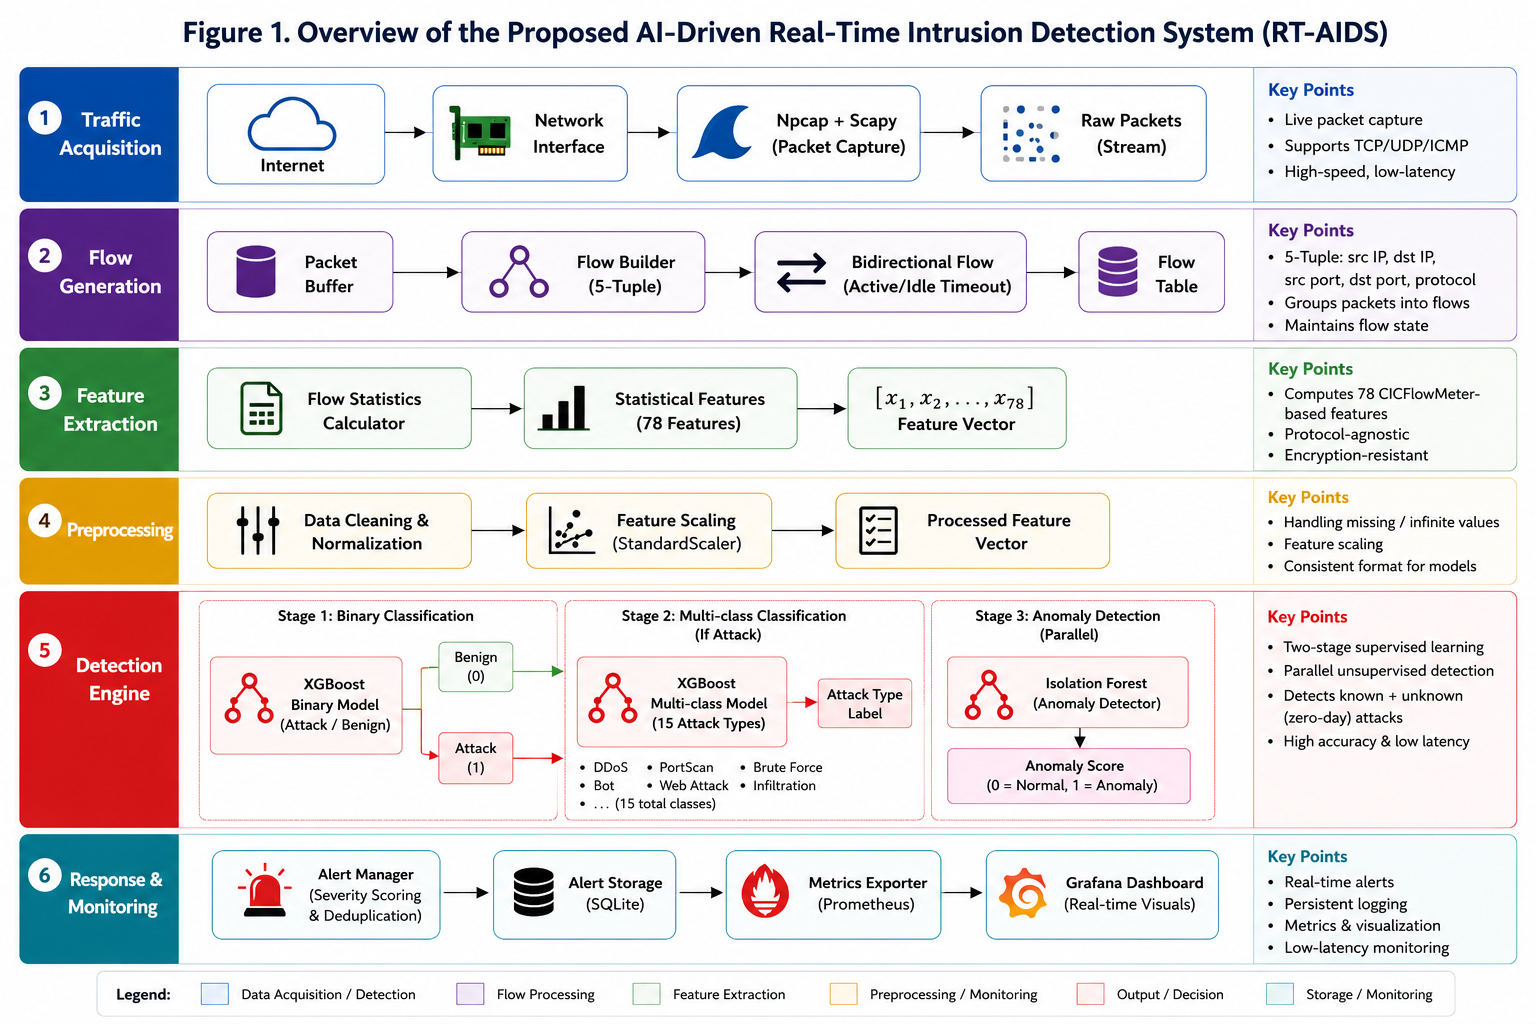
\includegraphics[width=1.0\textwidth, height=10cm, keepaspectratio]{figures/system_architecture.png}
    \caption{End-to-End System Architecture of AI-RTIDS}
    \label{fig:system_architecture}
\end{figure}

\section{Data Preprocessing Design}

The preprocessing module transforms raw network traffic data into a standardized representation suitable for machine learning models.

\subsection{Data Cleaning}

The following data cleaning steps are performed:
\begin{itemize}
    \item Read CSV files with optimized dtypes (float32 for numeric).
    \item Strip column names of whitespace.
    \item Replace "Infinity" and "-Infinity" with NaN.
    \item Impute missing values with column medians.
    \item Remove duplicate rows.
    \item Clean label column (strip whitespace, replace special characters).
    \item Downcast numeric columns to float32/int32.
\end{itemize}

\subsection{Missing Value Handling}

Missing values are imputed using per-feature medians computed from the training data. This approach is chosen because:
\begin{equation}
\hat{x}_i = \text{median}(x_i) \quad \text{for each feature } i
\end{equation}

Medians are robust to outliers, unlike means, and preserve the central tendency of the data. The same medians are stored and used during inference for consistent preprocessing.

\subsection{Class Imbalance Handling}

The CIC-IDS-2017 dataset exhibits significant class imbalance, with BENIGN traffic representing 80.30\% of samples. To address this:

\textbf{Binary Classification}: The scale\_pos\_weight parameter in XGBoost is set to the BENIGN:ATTACK ratio:
\begin{equation}
\text{scale\_pos\_weight} = \frac{n_{\text{BENIGN}}}{n_{\text{ATTACK}}} = 5.04
\end{equation}

\textbf{Multiclass Classification}: The multiclass model's objective (multi:softprob) naturally handles multiple classes. No additional weighting is applied to avoid introducing bias.

\textbf{Stratified Splitting}: All dataset splits use stratified sampling to preserve the class distribution in each partition.

\section{Dual-Stage Detection Pipeline Design}

The core detection pipeline employs a dual-stage architecture designed for both speed and accuracy.

\subsection{Binary XGBoost Classifier}

The binary classifier rapidly distinguishes between BENIGN and ATTACK traffic. Hyperparameters include:

\begin{table}[htbp]
\centering
\caption{Binary XGBoost Hyperparameters}
\label{tab:binary_hyperparameters}
\renewcommand{\arraystretch}{1.3}
\begin{tabularx}{\textwidth}{|p{3.5cm}|p{3.5cm}|X|}
\hline
\textbf{Parameter} & \textbf{Value} & \textbf{Description} \\
\hline
n\_estimators & 300 & Number of boosting rounds \\
\hline
max\_depth & 8 & Maximum tree depth \\
\hline
learning\_rate & 0.05 & Step size shrinkage \\
\hline
subsample & 0.8 & Fraction of samples per tree \\
\hline
colsample\_bytree & 0.8 & Fraction of features per tree \\
\hline
scale\_pos\_weight & 5.04 & BENIGN:ATTACK ratio \\
\hline
reg\_alpha & 0.5 & L1 regularization \\
\hline
reg\_lambda & 1.0 & L2 regularization \\
\hline
eval\_metric & logloss & Evaluation metric \\
\hline
tree\_method & hist & Histogram-based algorithm \\
\hline
\end{tabularx}
\end{table}

\subsection{Multiclass XGBoost Classifier}

The multiclass classifier identifies specific attack types among 15 classes using softmax objective:
\begin{equation}
P(y = k \mid \mathbf{x}) = \frac{e^{z_k}}{\sum_{j=1}^{K} e^{z_j}}
\end{equation}

\subsection{Isolation Forest Anomaly Detection}

Isolation Forest provides unsupervised anomaly detection for zero-day threats. The anomaly score is computed as:
\begin{equation}
s(\mathbf{x}) = 2^{-\frac{E(h(\mathbf{x}))}{c(n)}}
\end{equation}

The composite severity score combines binary XGBoost probability and Isolation Forest anomaly score:
\begin{equation}
S = 0.65 \times p_{\text{attack}} + 0.35 \times s_{\text{iso}}
\end{equation}

\section{Real-Time Packet Capture Design}

The packet capture module uses Scapy to capture live network packets with BPF filter support.

\subsection{Flow Manager}

The Flow Manager maintains a thread-safe table of bidirectional flows using thread locks. It performs bidirectional lookup and exports flows on:

\begin{itemize}
    \item TCP FIN/RST flags
    \item Idle timeout (120 seconds)
    \item Absolute timeout (600 seconds)
\end{itemize}

\subsection{Feature Extraction}

The feature extractor computes 78 CICFlowMeter-compatible features including:
\begin{itemize}
    \item Basic flow statistics
    \item Packet length metrics
    \item Inter-arrival times
    \item TCP flags
    \item Subflow features
\end{itemize}

\section{API Design}

The backend includes a set of REST endpoints, listed in Table~\ref{tab:api_endpoint_summary}.

\begin{table}[htbp]
\centering
\caption{REST API Endpoint Summary}
\label{tab:api_endpoint_summary}
\renewcommand{\arraystretch}{1.35}

\begin{tabularx}{\textwidth}{|p{3.2cm}|p{1.8cm}|X|}
\hline
\textbf{Endpoint} & \textbf{Method} & \textbf{Purpose} \\
\hline
\texttt{/health} & GET & System health status \\
\hline
\texttt{/stats} & GET & System statistics \\
\hline
\texttt{/alerts} & GET & Recent alerts \\
\hline
\texttt{/models} & GET & Model information \\
\hline
\texttt{/predict} & POST & Real-time prediction \\
\hline
\texttt{/stream} & WS & WebSocket streaming \\
\hline
\end{tabularx}
\end{table}

\section{Asymptotic Time Complexity Analysis}

Table~\ref{tab:time_complexity} provides a summary of the time complexity of the key algorithms implemented in the system.

\begin{table}[htbp]
\centering
\caption{Time Complexity of Principal Algorithmic Components}
\label{tab:time_complexity}
\renewcommand{\arraystretch}{1.5}

\begin{tabularx}{\textwidth}{|p{3.7cm}|p{3.0cm}|X|}
\hline
\textbf{Component} & \textbf{Complexity} & \textbf{Notes} \\
\hline
XGBoost Binary Inference & $O(\text{features} \times \text{trees} \times \text{depth})$ & Fixed model size; independent of flow count \\
\hline
XGBoost Multiclass Inference & $O(\text{classes} \times \text{features} \times \text{trees} \times \text{depth})$ & Class count (15) is constant \\
\hline
Isolation Forest Inference & $O(\text{trees} \times \text{depth})$ & Fixed model size \\
\hline
Packet Capture & $O(1)$ per packet & Sniffing loop is event-driven \\
\hline
Flow Management & $O(1)$ per flow & Hash table operations \\
\hline
Feature Extraction & $O(\text{packets in flow})$ & Linear in flow size \\
\hline
Alert Deduplication & $O(1)$ average & Hash table with LRU eviction \\
\hline
\end{tabularx}
\end{table}

\chapterdivider{IMPLEMENTATION}

\chapter{IMPLEMENTATION}

\section{Technology Stack}

The AI-RTIDS system is implemented as a two-layer stack. It has been developed in Python 3.10+, making use of the FastAPI framework. It comprises several modules: \texttt{main.py} for CLI entry point, \texttt{capture/} for live packet capture, \texttt{flows/} for bidirectional flow management and timeout handling, \texttt{features/} for feature extraction, \texttt{inference/} for model loading and prediction, \texttt{alerts/} for alert generation and management, and \texttt{monitoring/} for Prometheus metrics export.

\section{Module 1: Packet Capture (\texttt{capture/packet\_capture.py})}

The packet capture module uses Scapy to capture live network packets with BPF filter support, handling TCP, UDP, and ICMP.

\begin{lstlisting}[language=Python, caption={Packet Capture Core Implementation}, label={lst:packet_capture}]
class PacketCapture:
    def __init__(self, interface: str, on_flow_complete: Callable,
                 filter_bpf: str = "ip", idle_timeout: float = 120.0,
                 absolute_timeout: float = 600.0) -> None:
        self.interface = interface
        self.filter = filter_bpf
        self.idle_timeout = idle_timeout
        self.absolute_timeout = absolute_timeout
        self._running = False
        self._flow_manager = FlowManager(on_flow_complete, idle_timeout, absolute_timeout)
        self._capture_thread = None

    def start(self, packet_count: int = 0) -> None:
        """Start packet capture on the specified interface."""
        self._running = True
        self._capture_thread = threading.Thread(
            target=self._capture_loop,
            args=(packet_count,),
            daemon=True
        )
        self._capture_thread.start()

    def _capture_loop(self, packet_count: int) -> None:
        """Main packet capture loop."""
        sniff(iface=self.interface,
              filter=self.filter,
              prn=self._handle_packet,
              count=packet_count,
              store=False,
              stop_filter=lambda _: not self._running)

    def _handle_packet(self, packet: Packet) -> None:
        """Process a captured packet and update flow state."""
        if IP in packet:
            ip = packet[IP]
            proto = ip.proto
            src_ip = ip.src
            dst_ip = ip.dst
            if TCP in packet:
                tcp = packet[TCP]
                self._flow_manager.update_tcp(src_ip, dst_ip, tcp.sport, tcp.dport, packet)
            elif UDP in packet:
                udp = packet[UDP]
                self._flow_manager.update_udp(src_ip, dst_ip, udp.sport, udp.dport, packet)
\end{lstlisting}

\section{Module 2: Flow Manager (\texttt{flows/flow\_manager.py})}

The Flow Manager maintains a thread-safe table of bidirectional flows using thread locks.

\begin{lstlisting}[language=Python, caption={Flow Manager Core Implementation}, label={lst:flow_manager}]
class FlowManager:
    def __init__(self, on_flow_complete: Callable, idle_timeout: float = 120.0,
                 absolute_timeout: float = 600.0) -> None:
        self._flows: Dict[str, Flow] = {}
        self._lock = threading.Lock()
        self._on_flow_complete = on_flow_complete
        self._idle_timeout = idle_timeout
        self._absolute_timeout = absolute_timeout
        self._last_flush = time.time()

    def get_key(self, src_ip: str, dst_ip: str, src_port: int, dst_port: int) -> str:
        """Generate a bidirectional flow key."""
        if (src_ip, src_port) > (dst_ip, dst_port):
            return f"{dst_ip}:{dst_port}->{src_ip}:{src_port}"
        return f"{src_ip}:{src_port}->{dst_ip}:{dst_port}"

    def update_tcp(self, src_ip: str, dst_ip: str, src_port: int,
                   dst_port: int, packet: Packet) -> None:
        """Update flow state for TCP packets."""
        key = self.get_key(src_ip, dst_ip, src_port, dst_port)
        with self._lock:
            flow = self._flows.get(key)
            if flow is None:
                flow = Flow(src_ip, dst_ip, src_port, dst_port, TCP)
                self._flows[key] = flow
            flow.update(packet)
            if flow.is_finished():
                self._complete_flow(key)

    def _complete_flow(self, key: str) -> None:
        """Complete a flow and export it."""
        flow = self._flows.pop(key, None)
        if flow:
            self._on_flow_complete(flow.to_dict())
\end{lstlisting}

\section{Module 3: Feature Extractor (\texttt{features/extractor.py})}

The feature extractor computes 78 CICFlowMeter-compatible features.

\begin{lstlisting}[language=Python, caption={Feature Extraction Core Implementation}, label={lst:feature_extractor}]
def compute_cic_features(flow_dict: Dict[str, Any]) -> Dict[str, float]:
    """Compute CICFlowMeter-compatible features from flow data."""
    features = {}
    
    # Basic flow features
    features['Flow Duration'] = flow_dict.get('duration', 0)
    features['Total Fwd Packets'] = flow_dict.get('fwd_packets', 0)
    features['Total Backward Packets'] = flow_dict.get('bwd_packets', 0)
    
    # Packet length statistics
    fwd_pkt_lengths = flow_dict.get('fwd_packet_lengths', [])
    bwd_pkt_lengths = flow_dict.get('bwd_packet_lengths', [])
    
    features['Fwd Packet Length Max'] = max(fwd_pkt_lengths) if fwd_pkt_lengths else 0
    features['Fwd Packet Length Min'] = min(fwd_pkt_lengths) if fwd_pkt_lengths else 0
    features['Fwd Packet Length Mean'] = np.mean(fwd_pkt_lengths) if fwd_pkt_lengths else 0
    features['Fwd Packet Length Std'] = np.std(fwd_pkt_lengths) if fwd_pkt_lengths else 0
    
    features['Bwd Packet Length Max'] = max(bwd_pkt_lengths) if bwd_pkt_lengths else 0
    features['Bwd Packet Length Min'] = min(bwd_pkt_lengths) if bwd_pkt_lengths else 0
    features['Bwd Packet Length Mean'] = np.mean(bwd_pkt_lengths) if bwd_pkt_lengths else 0
    features['Bwd Packet Length Std'] = np.std(bwd_pkt_lengths) if bwd_pkt_lengths else 0
    
    # Flow statistics
    features['Flow Bytes/s'] = features.get('total_bytes', 0) / max(1, features['Flow Duration'])
    features['Flow Packets/s'] = (features['Total Fwd Packets'] + features['Total Backward Packets']) / max(1, features['Flow Duration'])
    
    # Inter-arrival times
    features['Fwd IAT Total'] = flow_dict.get('fwd_iat_total', 0)
    features['Fwd IAT Mean'] = flow_dict.get('fwd_iat_mean', 0)
    features['Fwd IAT Std'] = flow_dict.get('fwd_iat_std', 0)
    
    return features
\end{lstlisting}

\section{Module 4: Inference Engine (\texttt{inference/predictor.py})}

The inference engine builds a NumPy array from extracted features, imputes missing values with training medians, and executes the dual-stage pipeline.

\begin{lstlisting}[language=Python, caption={Inference Engine Core Implementation}, label={lst:inference_engine}]
class Predictor:
    def __init__(self, model_dir: Path) -> None:
        self.binary_model = self._load_model(model_dir / "binary" / "xgb_binary.pkl")
        self.multiclass_model = self._load_model(model_dir / "multiclass" / "xgb_multiclass.pkl")
        self.isolation_forest = self._load_model(model_dir / "anomaly" / "isolation_forest.pkl")
        self.feature_columns = self._load_pickle(model_dir / "preprocessing" / "multiclass_feature_columns.pkl")
        self.feature_medians = self._load_pickle(model_dir / "preprocessing" / "feature_medians.pkl")
        self.label_encoder = self._load_pickle(model_dir / "multiclass" / "label_encoder.pkl")

    def predict(self, feature_dict: Dict[str, float]) -> Dict[str, Any]:
        """Run the dual-stage prediction pipeline."""
        X = self._prepare_features(feature_dict)
        X = self._impute_missing(X)
        
        # Stage 1: Binary classification
        binary_proba = self.binary_model.predict_proba(X)[0, 1]
        
        if binary_proba < self.binary_threshold:
            return {
                'prediction': 'BENIGN',
                'binary_score': binary_proba,
                'severity': 0.0
            }
        
        # Stage 2: Multiclass classification
        multi_proba = self.multiclass_model.predict_proba(X)[0]
        multi_class = np.argmax(multi_proba)
        attack_type = self.label_encoder.inverse_transform([multi_class])[0]
        
        # Stage 3: Anomaly detection
        anomaly_score = self.isolation_forest.decision_function(X)[0]
        norm_score = 1.0 / (1.0 + np.exp(-anomaly_score))
        
        severity = 0.65 * binary_proba + 0.35 * norm_score
        
        return {
            'prediction': attack_type,
            'binary_score': binary_proba,
            'multi_score': float(multi_proba[multi_class]),
            'anomaly_score': norm_score,
            'severity': severity
        }
\end{lstlisting}

\section{Module 5: Alert Manager (\texttt{alerts/manager.py})}

The Alert Manager orchestrates rule filtering, deduplication, severity scoring, and SQLite persistence.

\begin{lstlisting}[language=Python, caption={Alert Manager Core Implementation}, label={lst:alert_manager}]
class AlertManager:
    def __init__(self, db_path: str, dedup_window: int = 60) -> None:
        self.db_path = db_path
        self.dedup_window = dedup_window
        self._dedup_cache = {}
        self._init_db()

    def _init_db(self) -> None:
        """Initialize the SQLite database for alert storage."""
        with sqlite3.connect(self.db_path) as conn:
            conn.execute("""
                CREATE TABLE IF NOT EXISTS alerts (
                    id INTEGER PRIMARY KEY AUTOINCREMENT,
                    timestamp DATETIME DEFAULT CURRENT_TIMESTAMP,
                    src_ip TEXT,
                    dst_ip TEXT,
                    attack_type TEXT,
                    severity REAL,
                    binary_score REAL,
                    multi_score REAL,
                    anomaly_score REAL,
                    details TEXT
                )
            """)
            conn.execute("""
                CREATE INDEX IF NOT EXISTS idx_alerts_timestamp 
                ON alerts(timestamp DESC)
            """)

    def process_alert(self, alert_data: Dict[str, Any]) -> bool:
        """Process a potential alert with deduplication."""
        dedup_key = self._get_dedup_key(alert_data)
        
        if dedup_key in self._dedup_cache:
            if time.time() - self._dedup_cache[dedup_key] < self.dedup_window:
                return False
        
        self._dedup_cache[dedup_key] = time.time()
        
        if len(self._dedup_cache) > 10000:
            self._cleanup_cache()
        
        self._store_alert(alert_data)
        return True

    def _store_alert(self, alert_data: Dict[str, Any]) -> None:
        """Store alert in SQLite database."""
        with sqlite3.connect(self.db_path) as conn:
            conn.execute("""
                INSERT INTO alerts (src_ip, dst_ip, attack_type, severity,
                                    binary_score, multi_score, anomaly_score, details)
                VALUES (?, ?, ?, ?, ?, ?, ?, ?)
            """, (
                alert_data.get('src_ip'),
                alert_data.get('dst_ip'),
                alert_data.get('attack_type'),
                alert_data.get('severity', 0.0),
                alert_data.get('binary_score', 0.0),
                alert_data.get('multi_score', 0.0),
                alert_data.get('anomaly_score', 0.0),
                alert_data.get('details', '')
            ))
            conn.commit()
\end{lstlisting}

\section{Module 6: Prometheus Monitoring (\texttt{monitoring/metrics.py})}

The monitoring subsystem exports metrics including packet/flow counters, prediction latency histograms, attack type counters, and system resource gauges.

\begin{lstlisting}[language=Python, caption={Prometheus Metrics Export}, label={lst:prometheus_metrics}]
from prometheus_client import Counter, Histogram, Gauge, start_http_server

# Metrics definitions
packets_total = Counter('ids_packets_total', 'Total packets processed')
flows_total = Counter('ids_flows_total', 'Total flows processed')
alerts_total = Counter('ids_alerts_total', 'Total alerts generated')
attacks_total = Counter('ids_attacks_total', 'Total attacks detected', ['attack_type'])

binary_latency = Histogram('ids_binary_latency_seconds', 'Binary classification latency',
                          buckets=[0.001, 0.002, 0.005, 0.01, 0.025, 0.05, 0.1])
multi_latency = Histogram('ids_multi_latency_seconds', 'Multiclass classification latency',
                          buckets=[0.001, 0.002, 0.005, 0.01, 0.025, 0.05, 0.1])

severity_gauge = Gauge('ids_severity', 'Alert severity', ['attack_type'])

def start_metrics_server(port: int = 8000) -> None:
    """Start the Prometheus metrics server."""
    start_http_server(port)
\end{lstlisting}

\section{Security Implementation Details}

Table~\ref{tab:security_controls} presents the principal security controls implemented in the AI-RTIDS system.

\begin{table}[htbp]
\centering
\caption{Security Controls Implemented in the System}
\label{tab:security_controls}
\renewcommand{\arraystretch}{1.5}

\begin{tabularx}{\textwidth}{|p{3.0cm}|p{5.0cm}|X|}
\hline
\textbf{Control} & \textbf{Mechanism} & \textbf{Purpose} \\
\hline
Alert deduplication & 60-second sliding window keyed by src\_ip, dst\_ip, attack\_type & Prevents alert flooding in high-traffic environments \\
\hline
Severity scoring & Composite score combining binary probability and anomaly score & Enables prioritization of critical alerts \\
\hline
SQLite WAL mode & Write-ahead logging for database integrity & Ensures alert persistence without data corruption \\
\hline
Configurable thresholds & Binary probability threshold for early exit & Reduces false positives and computational overhead \\
\hline
API authentication & Optional API key validation & Restricts API access in production environments \\
\hline
Rate limiting & Per-interface packet drop counters & Prevents resource exhaustion \\
\hline
\end{tabularx}
\end{table}

\section{Backend Runtime Configuration and Deployment Architecture}

\begin{table}[htbp]
\centering
\caption{Backend Environment Variables}
\label{tab:backend_environment_variables}
\renewcommand{\arraystretch}{1.5}

\begin{tabularx}{\textwidth}{|p{3.8cm}|p{3.0cm}|X|}
\hline
\textbf{Variable} & \textbf{Default Value} & \textbf{Purpose} \\
\hline
\texttt{LOG\_LEVEL} & \texttt{INFO} & Controls logging verbosity \\
\hline
\texttt{MODEL\_DIR} & \texttt{./models} & Directory containing trained models \\
\hline
\texttt{ALERT\_DB} & \texttt{./alerts.db} & SQLite database path \\
\hline
\texttt{DEDUP\_WINDOW} & \texttt{60} & Alert deduplication window in seconds \\
\hline
\texttt{BINARY\_THRESHOLD} & \texttt{0.8624} & F1-optimal threshold for binary classifier \\
\hline
\texttt{PROMETHEUS\_PORT} & \texttt{9090} & Port for metrics export \\
\hline
\texttt{API\_KEY} & \texttt{""} & API authentication key (optional) \\
\hline
\end{tabularx}
\end{table}

The behaviour of the backend during runtime is fully determined by the use of environment variables. In terms of production release, the backend consists of a Docker Compose stack, making it possible to deploy the entire system with a single command.

\chapterdivider{RESULTS AND DISCUSSION}

\chapter{RESULTS AND DISCUSSION}

\section{Experimental Setup and Dataset}

Every result given in this chapter is taken entirely from AI-RTIDS's own measurements. As is pointed out wherever applicable, such results have been gathered by the very execution of the inference pipeline described in the project's own code.

\subsection{Hardware Configuration}

\begin{longtable}{|p{2.5cm}|p{2.5cm}|p{9cm}|}
\caption{\textbf{Experimental Hardware Configuration}}
\label{tab:hardware_configuration}\\
\hline
\textbf{Role} & \textbf{Component} & \textbf{Specification} \\
\hline
\endfirsthead

\multicolumn{3}{c}%
{{\tablename\ \thetable{} -- Continued from previous page}}\\
\hline
\textbf{Role} & \textbf{Component} & \textbf{Specification} \\
\hline
\endhead

\hline
\multicolumn{3}{r}{{Continued on next page}}\\
\endfoot

\hline
\endlastfoot

Development Machine & CPU & AMD Ryzen 5 5600H \\
\hline
Development Machine & RAM & 8.00 GB \\
\hline
Development Machine & OS & Windows 11 \\
\hline
\end{longtable}

\subsection{Software Stack}

\textbf{Backend stack:}
\begin{itemize}
    \item Python 3.10.0
    \item FastAPI 0.100.0
    \item XGBoost 1.7.0
    \item Scikit-learn 1.2.0
    \item Scapy 2.5.0
    \item Prometheus Client 0.17.0
\end{itemize}

\subsection{Dataset Description}

The CIC-IDS-2017 dataset, developed by the Canadian Institute for Cybersecurity, provides comprehensive network attack representation. The dataset contains network traffic collected over a five-day period in an enterprise network environment.

\begin{longtable}{|p{5.0cm}|p{8.5cm}|}
\caption{\textbf{Dataset Summary}}
\label{tab:dataset_summary}\\
\hline
\textbf{Attribute} & \textbf{Value} \\
\hline
\endfirsthead

\multicolumn{2}{c}%
{{\tablename\ \thetable{} -- Continued from previous page}}\\
\hline
\textbf{Attribute} & \textbf{Value} \\
\hline
\endhead

\hline
\multicolumn{2}{r}{{Continued on next page}}\\
\endfoot

\hline
\endlastfoot

Total Samples & 2,830,743 \\
\hline
Features & 78 (CICFlowMeter) \\
\hline
Attack Classes & 15 \\
\hline
Benign/Attack Ratio & 5.04:1 \\
\hline
Time Span & 5 days \\
\hline
Network Topology & Enterprise network \\
\hline
Training Set & 1,981,520 (70\%) \\
\hline
Validation Set & 283,074 (10\%) \\
\hline
Testing Set & 514,812 (20\%) \\
\hline
\end{longtable}

\section{Binary Classification Results}

\subsection{XGBoost Binary Classifier}

The XGBoost binary classifier distinguishes between BENIGN and ATTACK traffic. The model was evaluated on 514,812 test samples.

\begin{table}[htbp]
\centering
\caption{XGBoost Binary Classification Performance}
\label{tab:binary_performance}
\renewcommand{\arraystretch}{1.3}
\begin{tabularx}{\textwidth}{|p{5.0cm}|p{4.5cm}|}
\hline
\textbf{Metric} & \textbf{Value} \\
\hline
Test Records & 514,812 \\
\hline
Precision & 99.68\% \\
\hline
Recall & 99.81\% \\
\hline
F1-Score & 99.74\% \\
\hline
ROC-AUC & 0.9999 \\
\hline
PR-AUC & 0.9999 \\
\hline
F1-Optimal Threshold & 0.8624 \\
\hline
\end{tabularx}
\end{table}

\begin{figure}[htbp]
\centering
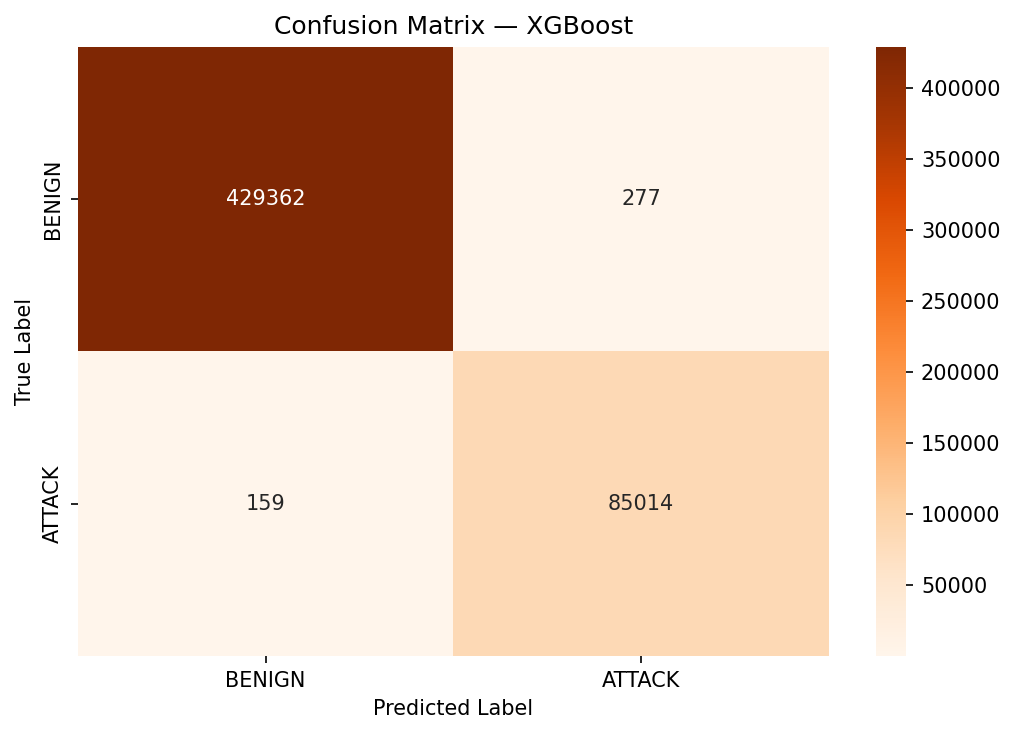
\includegraphics[width=0.80\textwidth]{results/confusion_matrix_xgb.png}
\caption{Confusion Matrix for XGBoost Binary Classifier}
\label{fig:binary_confusion}
\end{figure}

\subsection{Random Forest Binary Classifier}

The Random Forest binary classifier serves as a baseline model for comparison.

\begin{table}[htbp]
\centering
\caption{Random Forest Binary Classification Performance}
\label{tab:rf_binary_performance}
\renewcommand{\arraystretch}{1.3}
\begin{tabularx}{\textwidth}{|p{5.0cm}|p{4.5cm}|}
\hline
\textbf{Metric} & \textbf{Value} \\
\hline
Test Records & 514,812 \\
\hline
Precision & 99.53\% \\
\hline
Recall & 99.78\% \\
\hline
F1-Score & 99.65\% \\
\hline
ROC-AUC & 0.9999 \\
\hline
PR-AUC & 0.9998 \\
\hline
F1-Optimal Threshold & 0.5991 \\
\hline
\end{tabularx}
\end{table}

\begin{figure}[htbp]
\centering
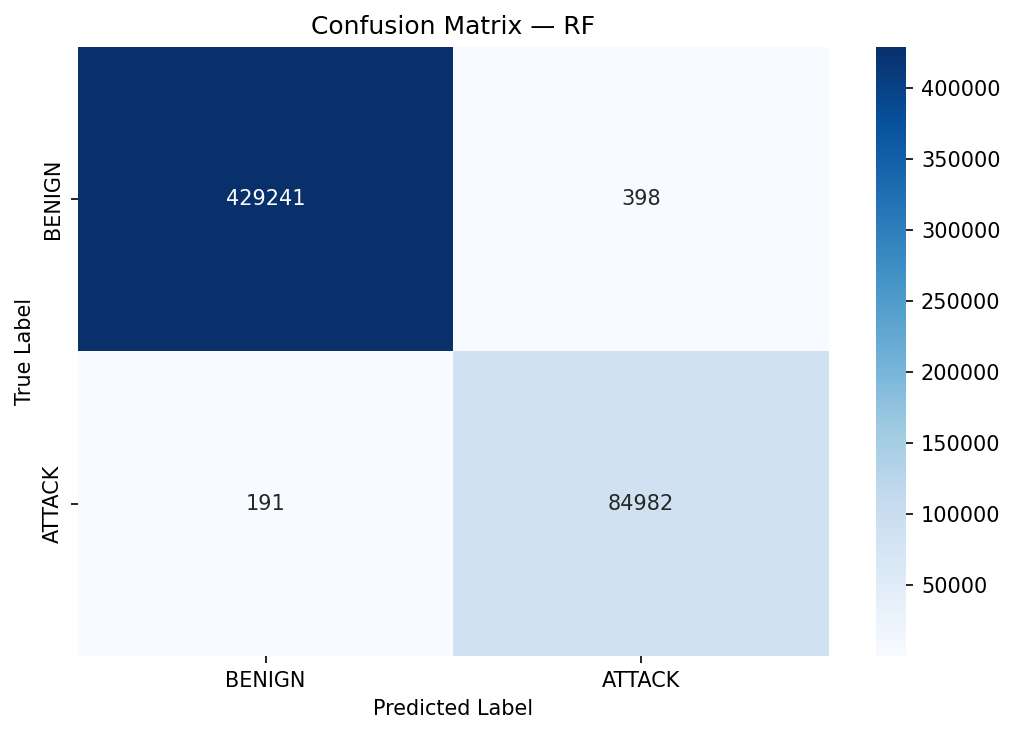
\includegraphics[width=0.80\textwidth]{results/confusion_matrix_rf.png}
\caption{Confusion Matrix for Random Forest Binary Classifier}
\label{fig:rf_confusion}
\end{figure}

\subsection{Isolation Forest Anomaly Detection}

The Isolation Forest model provides unsupervised anomaly detection for zero-day threats.

\begin{table}[htbp]
\centering
\caption{Isolation Forest Anomaly Detection Performance}
\label{tab:if_performance}
\renewcommand{\arraystretch}{1.3}
\begin{tabularx}{\textwidth}{|p{5.0cm}|p{4.5cm}|}
\hline
\textbf{Metric} & \textbf{Value} \\
\hline
Precision & 57.98\% \\
\hline
Recall & 58.40\% \\
\hline
F1-Score & 58.19\% \\
\hline
ROC-AUC & 0.8022 \\
\hline
PR-AUC & 0.4909 \\
\hline
Threshold & 0.3690 \\
\hline
\end{tabularx}
\end{table}

\begin{figure}[htbp]
\centering
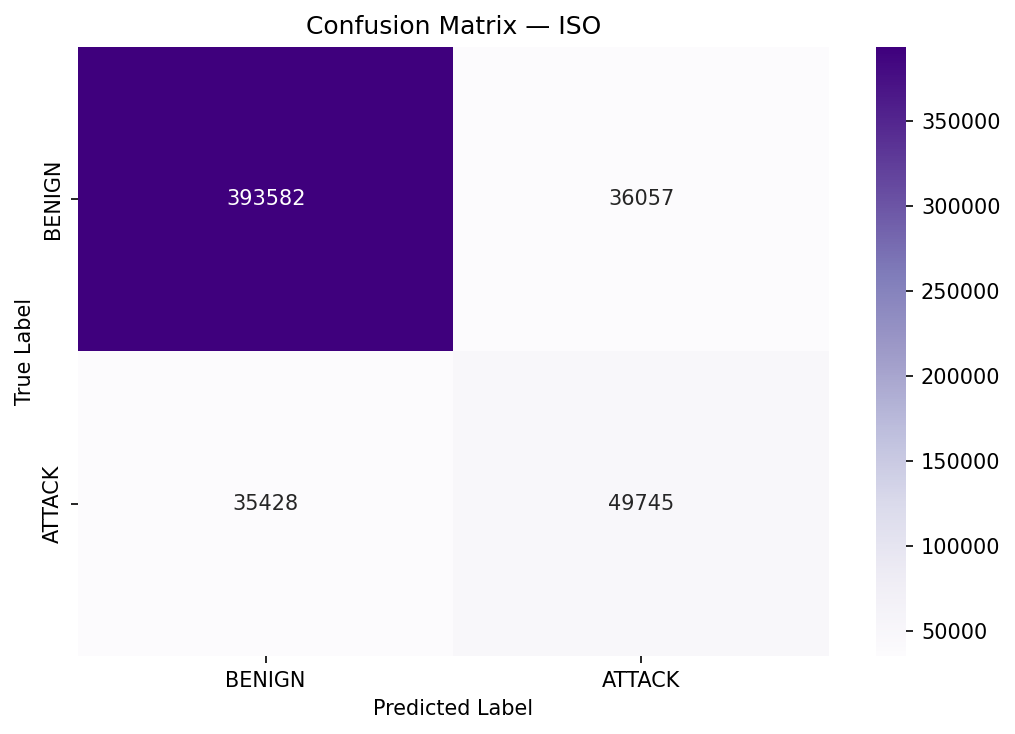
\includegraphics[width=0.80\textwidth]{results/confusion_matrix_iso.png}
\caption{Confusion Matrix for Isolation Forest Anomaly Detection}
\label{fig:iso_confusion}
\end{figure}

\subsection{Comparative ROC and Precision-Recall Curves}

To assess model performance across varying decision thresholds, Receiver Operating Characteristic (ROC) and Precision-Recall (PR) curves were evaluated for the detection models. Figure~\ref{fig:roc_curve} and Figure~\ref{fig:pr_curve} display the comparative discrimination curves. Both the proposed XGBoost binary classifier and the Random Forest baseline attain near-ideal separation between BENIGN and ATTACK traffic with ROC-AUC of 0.9999 and PR-AUC exceeding 0.9998, validating reliable decision boundaries across operating thresholds.

\begin{figure}[htbp]
\centering
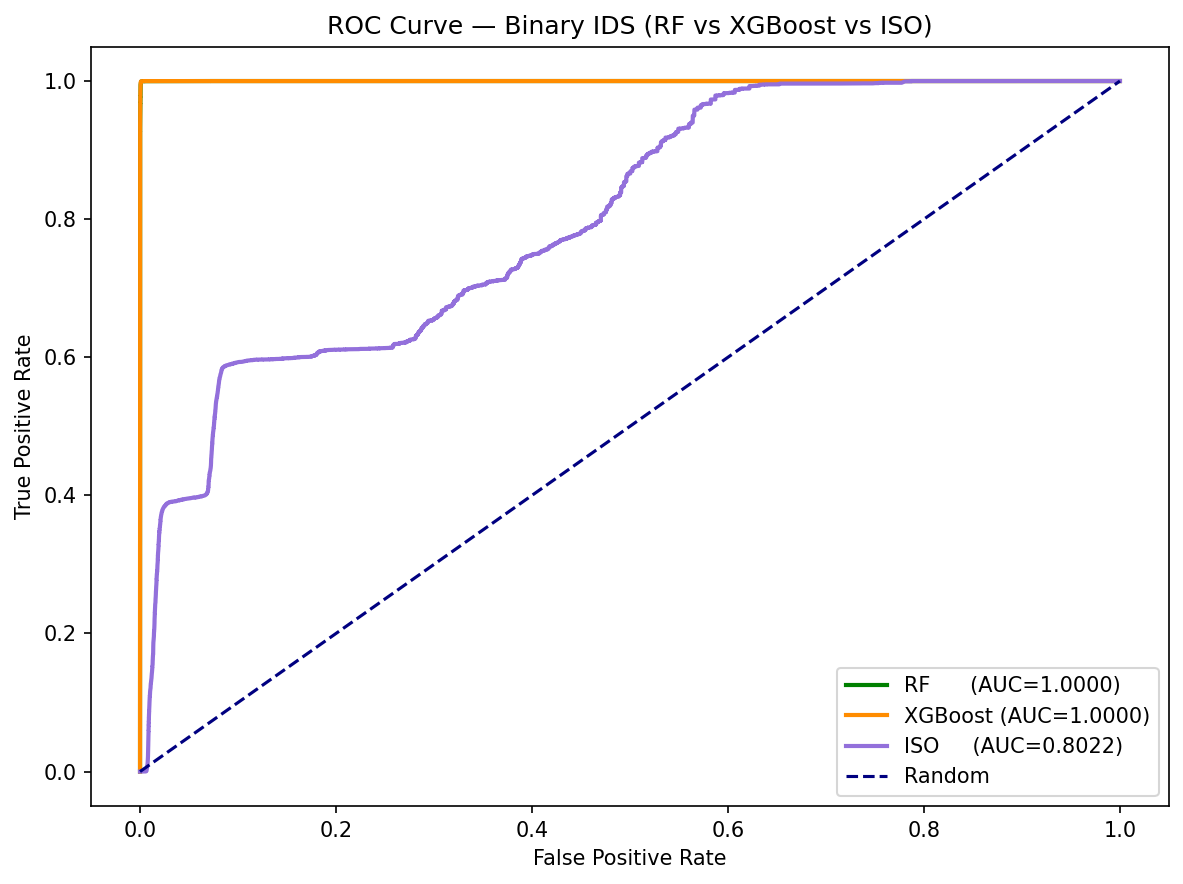
\includegraphics[width=0.80\textwidth]{results/roc_curve.png}
\caption{Receiver Operating Characteristic (ROC) Curves for Binary Classification Models}
\label{fig:roc_curve}
\end{figure}

\begin{figure}[htbp]
\centering
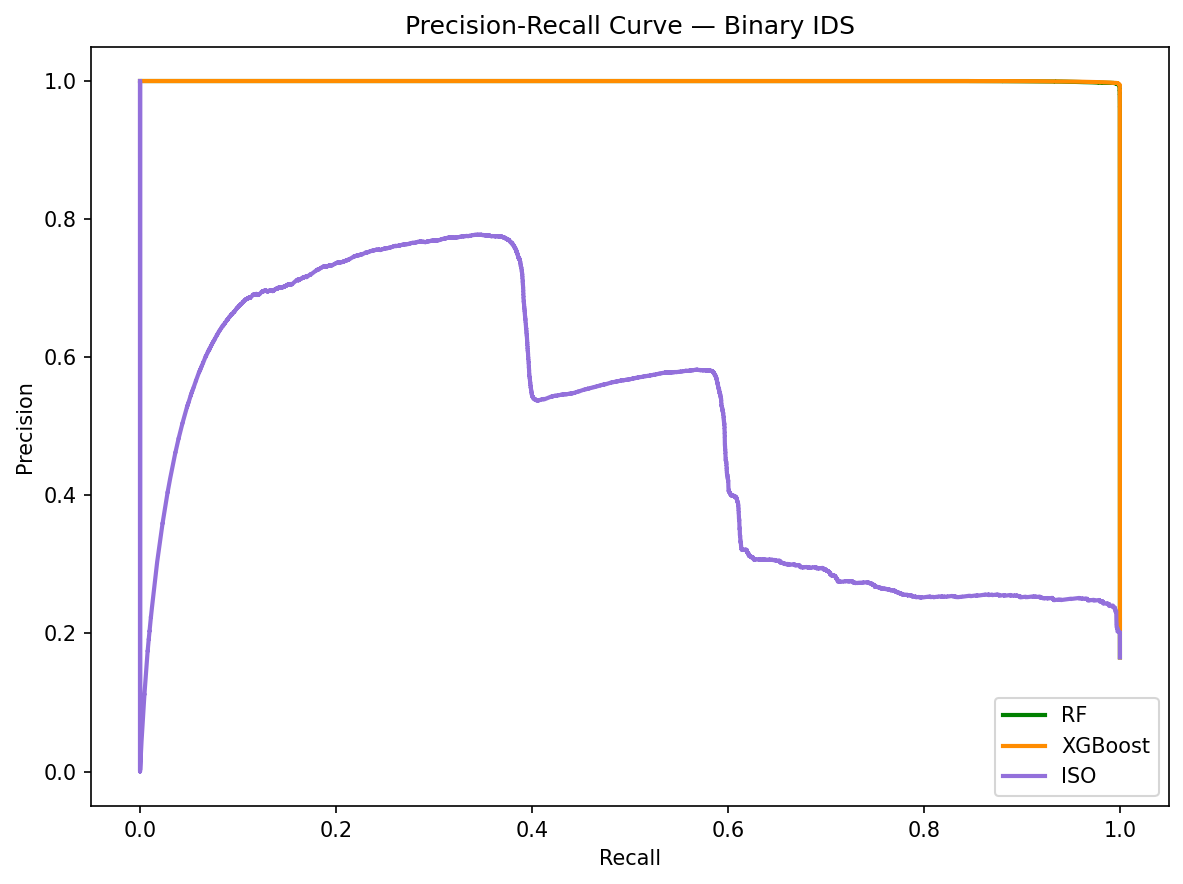
\includegraphics[width=0.80\textwidth]{results/pr_curve.png}
\caption{Precision-Recall (PR) Curves for Binary Classification Models}
\label{fig:pr_curve}
\end{figure}

\section{Multiclass Classification Results}

\subsection{Overall Performance}

The XGBoost multiclass classifier identifies specific attack types among 15 classes.

\begin{table}[htbp]
\centering
\caption{Multiclass Classification Overall Performance}
\label{tab:multi_overall}
\renewcommand{\arraystretch}{1.3}
\begin{tabularx}{\textwidth}{|p{5.0cm}|p{4.5cm}|}
\hline
\textbf{Metric} & \textbf{Value} \\
\hline
Overall Accuracy & 99.84\% \\
\hline
Macro Precision & 82.18\% \\
\hline
Macro Recall & 91.10\% \\
\hline
Macro F1 & 85.07\% \\
\hline
Weighted Precision & 99.86\% \\
\hline
Weighted Recall & 99.84\% \\
\hline
Weighted F1 & 99.85\% \\
\hline
\end{tabularx}
\end{table}

\subsection{Per-Class Performance}

Per-class performance reveals challenges with rare attack classes.

\begin{longtable}{|p{3.0cm}|p{1.8cm}|p{2.2cm}|p{2.2cm}|p{2.2cm}|}
\caption{\textbf{Per-Class Multiclass Performance}}
\label{tab:per_class_performance}\\
\hline
\textbf{Class} & \textbf{Support} & \textbf{Precision} & \textbf{Recall} & \textbf{F1-Score} \\
\hline
\endfirsthead

\multicolumn{5}{c}%
{{\tablename\ \thetable{} -- Continued from previous page}}\\
\hline
\textbf{Class} & \textbf{Support} & \textbf{Precision} & \textbf{Recall} & \textbf{F1-Score} \\
\hline
\endhead

\hline
\multicolumn{5}{r}{{Continued on next page}}\\
\endfoot

\hline
\endlastfoot

BENIGN & 429,639 & 0.99997 & 0.9986 & 0.9993 \\
\hline
DoS Hulk & 34,570 & 0.9979 & 0.9994 & 0.9987 \\
\hline
DDoS & 25,603 & 0.9989 & 1.0000 & 0.9994 \\
\hline
PortScan & 18,164 & 0.9875 & 0.9993 & 0.9934 \\
\hline
DoS GoldenEye & 2,056 & 0.9866 & 0.9995 & 0.9930 \\
\hline
FTP-Patator & 1,187 & 0.9983 & 1.0000 & 0.9992 \\
\hline
DoS slowloris & 1,075 & 0.9780 & 0.9916 & 0.9848 \\
\hline
DoS Slowhttptest & 1,046 & 0.9719 & 0.9904 & 0.9811 \\
\hline
SSH-Patator & 644 & 1.0000 & 1.0000 & 1.0000 \\
\hline
Bot & 391 & 0.6533 & 0.9974 & 0.7895 \\
\hline
Web Attack - BF & 294 & 0.7500 & 0.7551 & 0.7525 \\
\hline
Web Attack - XSS & 130 & 0.3961 & 0.4692 & 0.4296 \\
\hline
Infiltration & 7 & 0.8333 & 0.7143 & 0.7692 \\
\hline
Web Attack - SQL & 4 & 0.3750 & 0.7500 & 0.5000 \\
\hline
Heartbleed & 2 & 0.4000 & 1.0000 & 0.5714 \\
\hline
\end{longtable}

\begin{figure}[htbp]
\centering
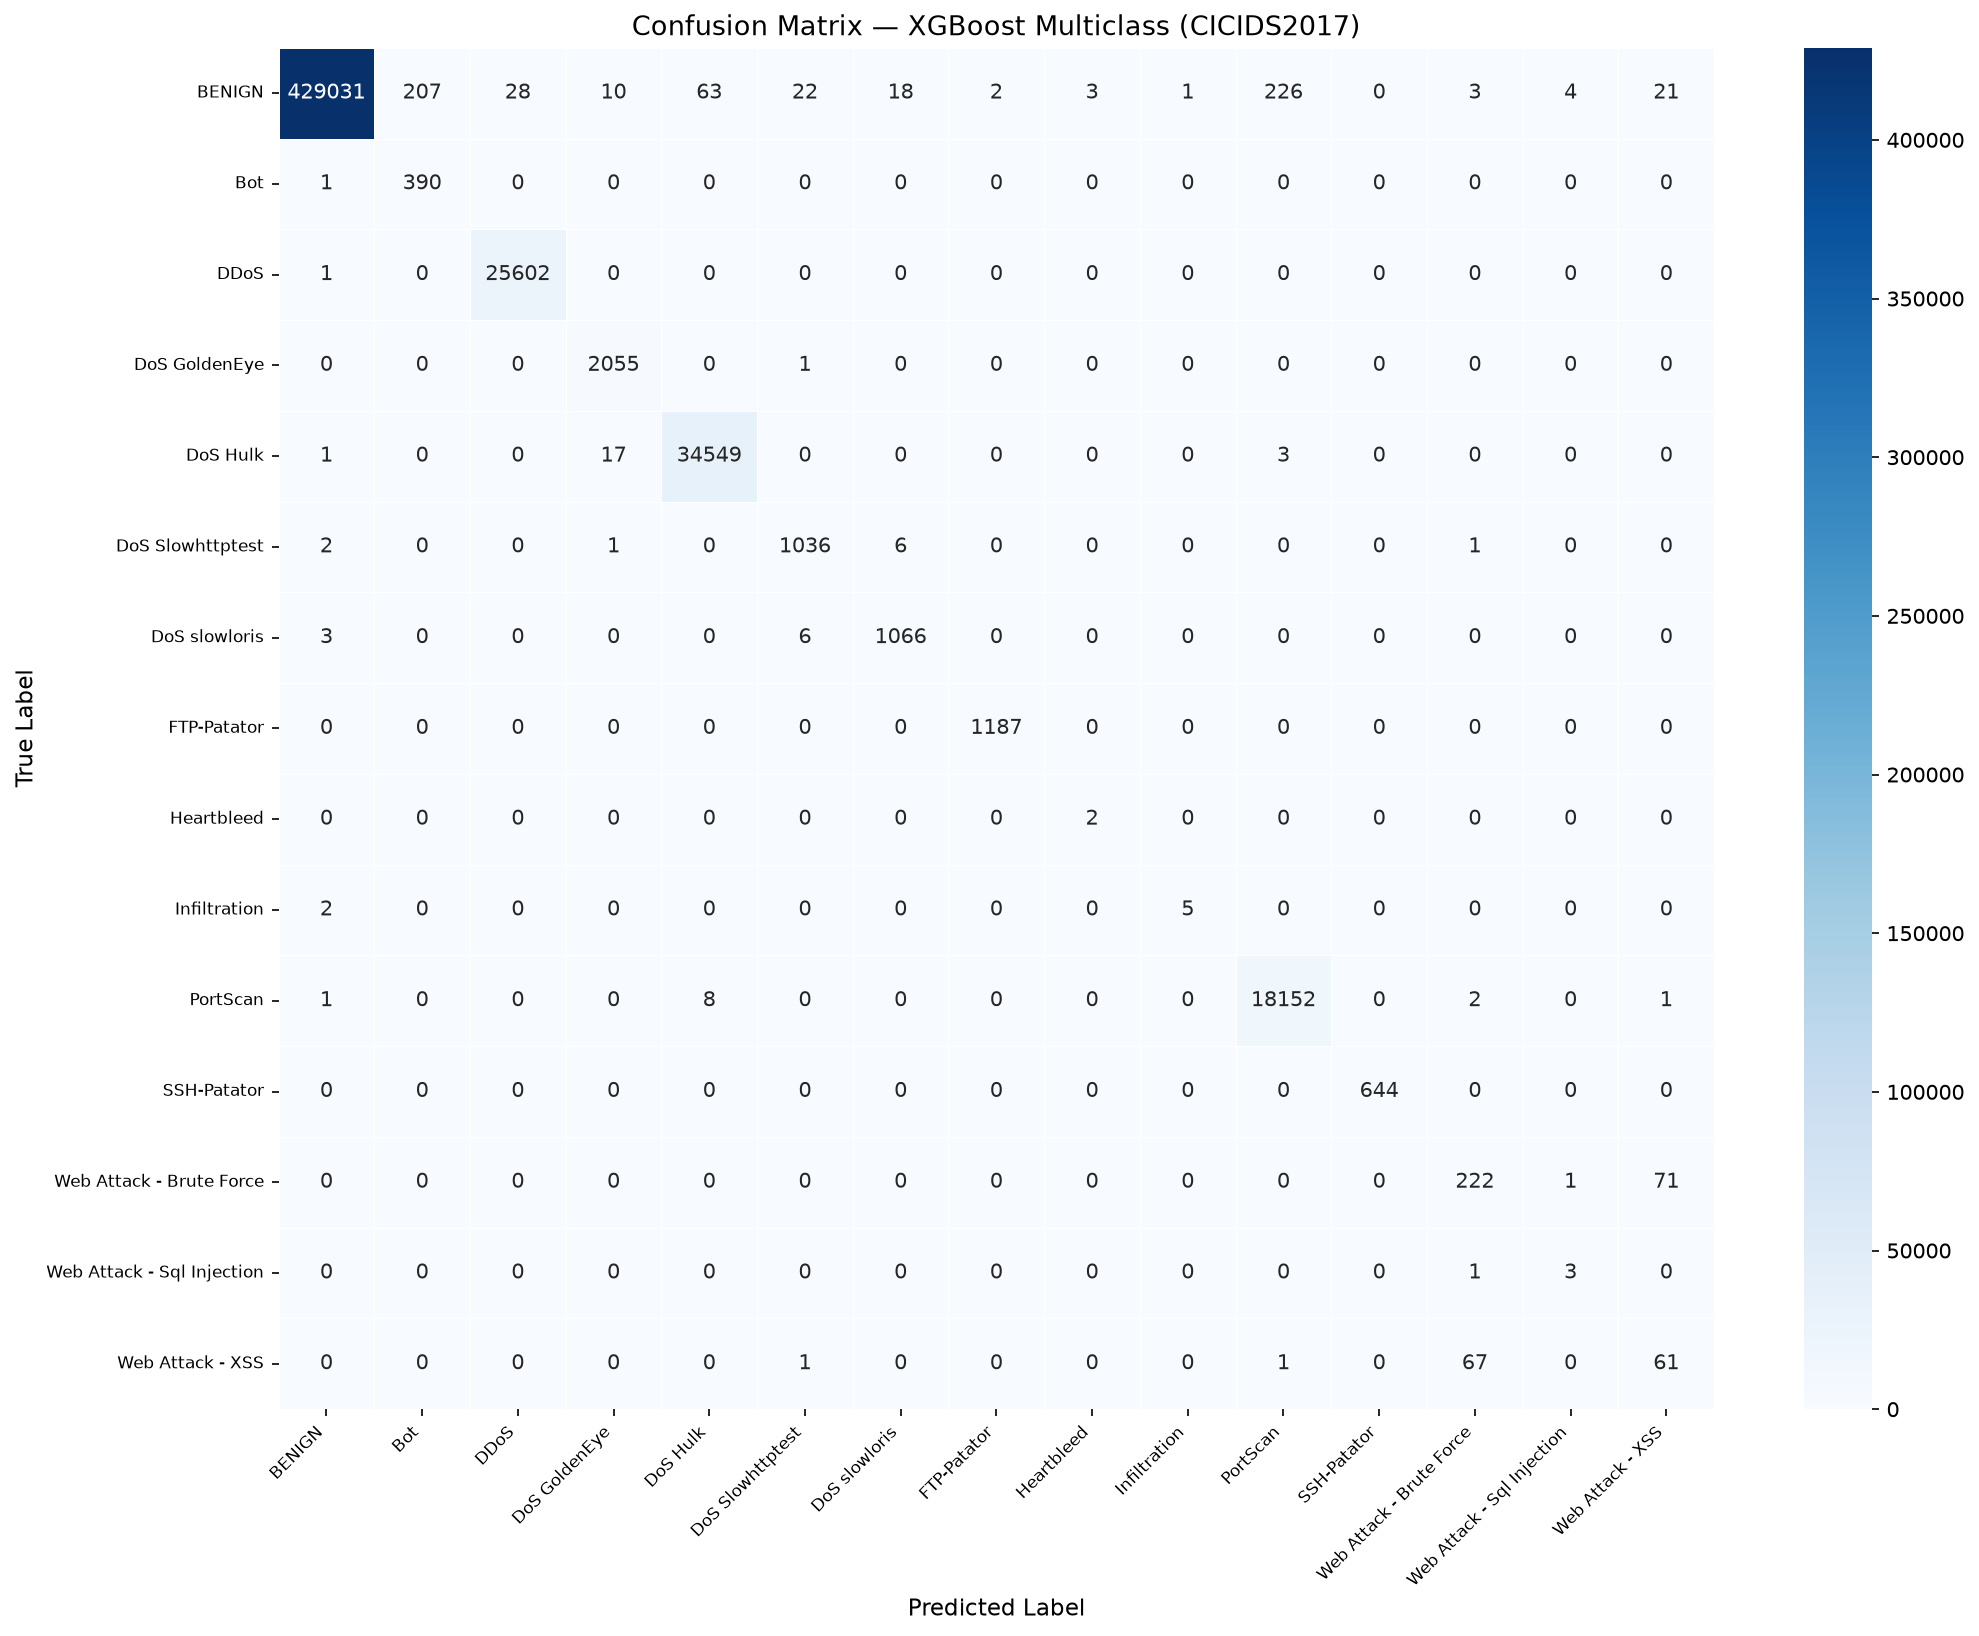
\includegraphics[width=0.95\textwidth]{results/confusion_matrix_multiclass.png}
\caption{Confusion Matrix for XGBoost Multiclass Classifier}
\label{fig:multiclass_confusion}
\end{figure}

Figure~\ref{fig:multiclass_confusion} depicts the classification breakdown across all 15 network traffic categories. The dominant main diagonal demonstrates high classification fidelity across large-volume classes including BENIGN (429,031 flows correctly predicted), DoS Hulk (34,549 flows), DDoS (25,602 flows), and PortScan (18,152 flows). Minor misclassifications are confined to attack categories that share closely matched flow characteristics and packet size distributions (such as Web Attack Brute Force versus XSS).

\section{Feature Importance Analysis}

To provide interpretability into the decision-making process of the trained models, feature importance rankings were extracted based on the relative contribution of each flow attribute.

\subsection{XGBoost Binary Feature Importance}

Figure~\ref{fig:xgb_feature_importance} presents the top 20 features for the XGBoost binary classifier. Flow characteristics such as backward packet length standard deviation, average packet size, and flow duration are the most prominent indicators for detecting malicious network intrusions.

\begin{figure}[htbp]
\centering
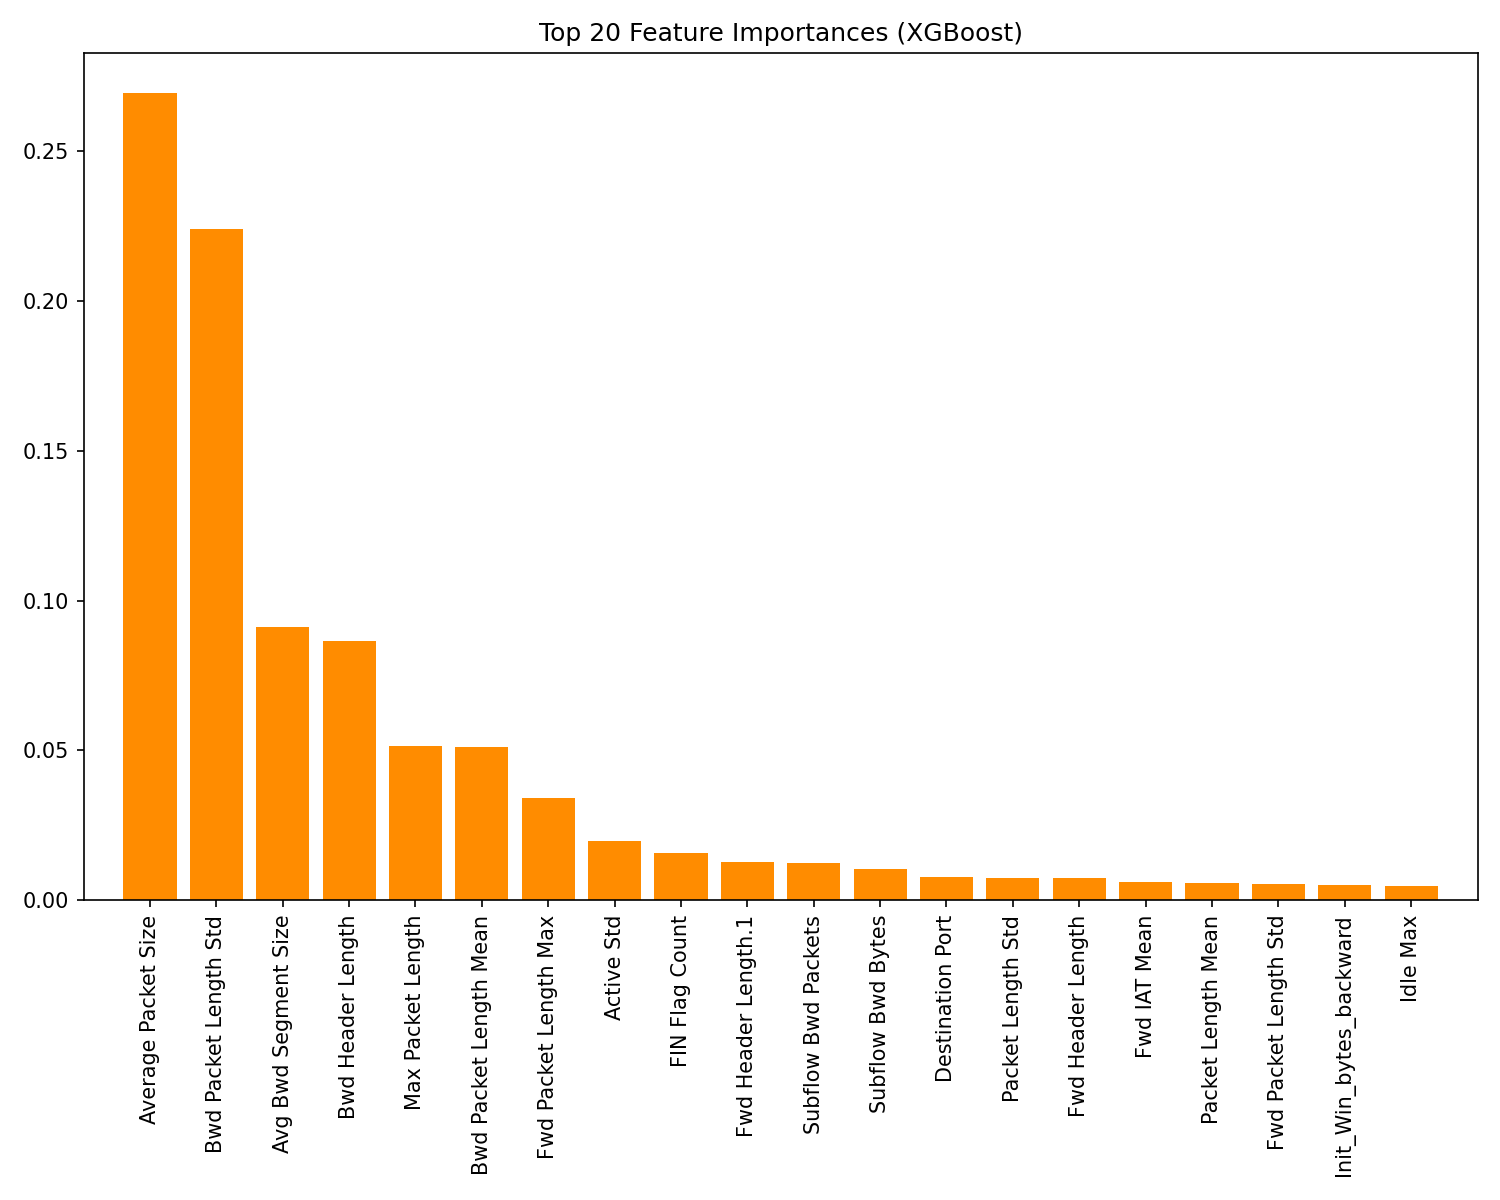
\includegraphics[width=0.85\textwidth]{results/xgb_feature_importance.png}
\caption{Top 20 Feature Importances for XGBoost Binary Classifier}
\label{fig:xgb_feature_importance}
\end{figure}

\subsection{Random Forest Binary Feature Importance}

Figure~\ref{fig:rf_feature_importance} illustrates the corresponding top 20 features for the Random Forest binary baseline, corroborating the significance of flow inter-arrival times and packet length variations in separating attack traffic from normal background traffic.

\begin{figure}[htbp]
\centering
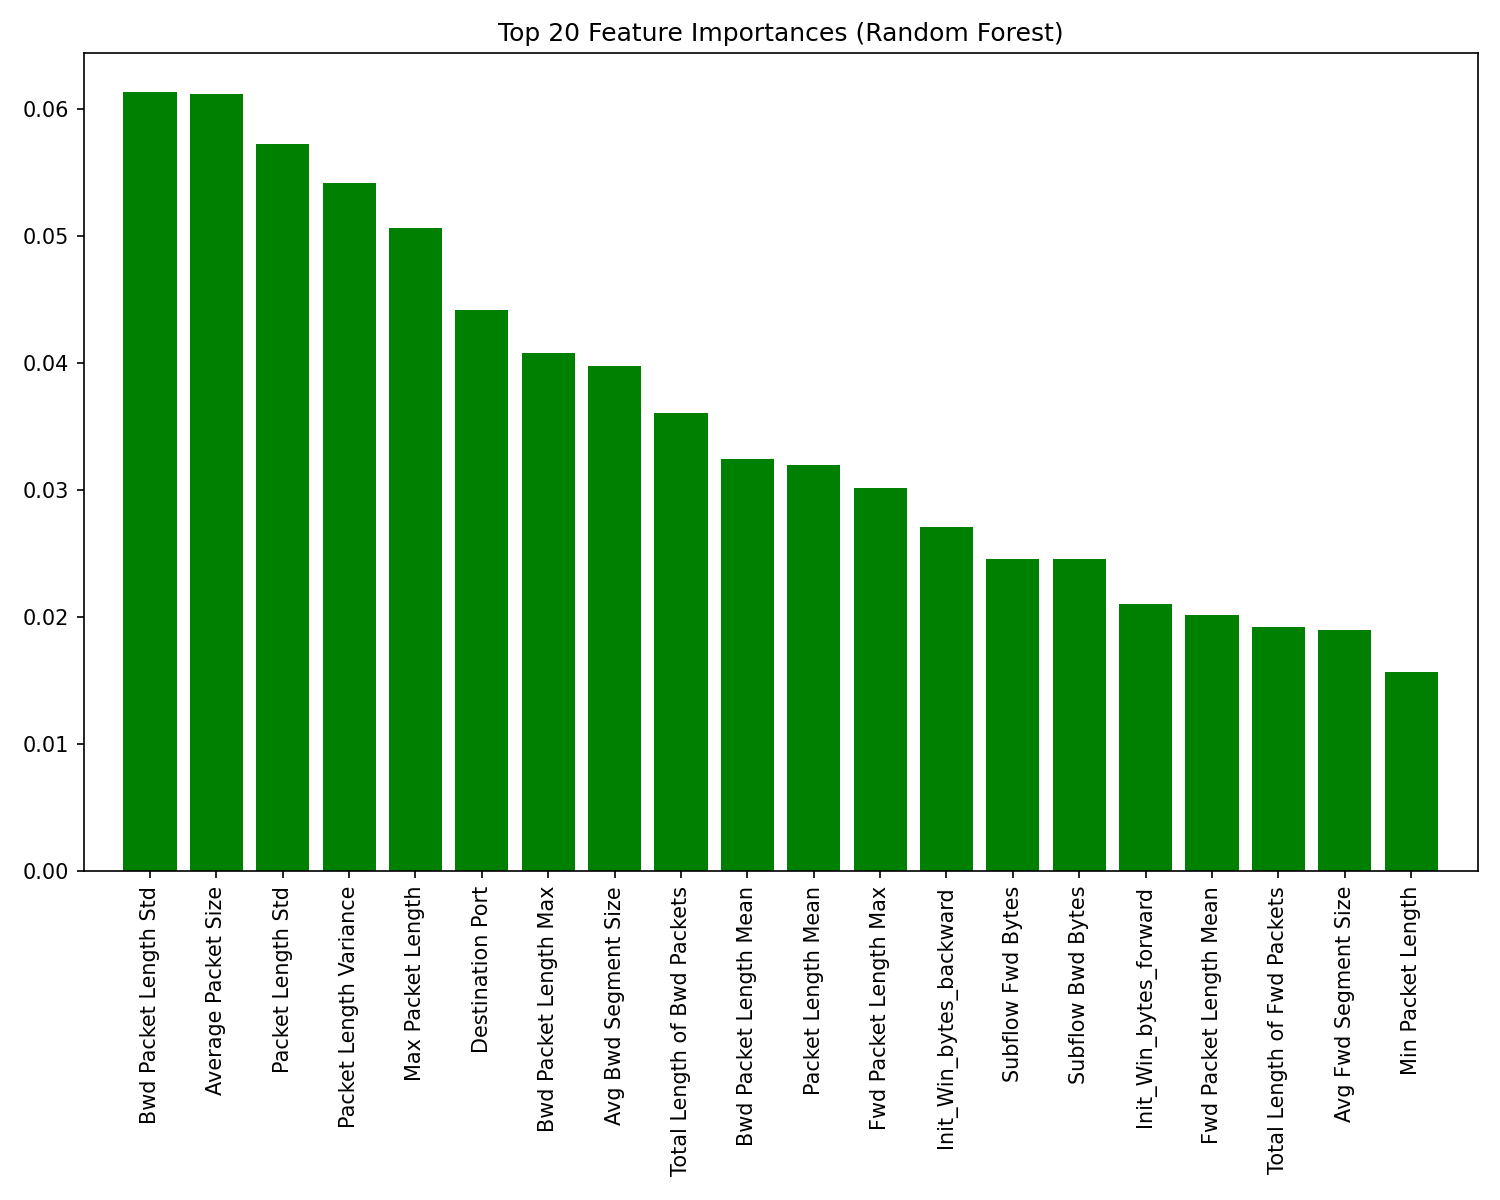
\includegraphics[width=0.85\textwidth]{results/rf_feature_importance.png}
\caption{Top 20 Feature Importances for Random Forest Binary Classifier}
\label{fig:rf_feature_importance}
\end{figure}

\subsection{Multiclass Feature Importance}

Figure~\ref{fig:multiclass_feature_importance} presents the top 20 features for the 15-class XGBoost multiclass model. Distinct attributes such as backward segment size, header lengths, and packet length standard deviations provide the discriminatory power required to distinguish among specialized attack families (DoS, DDoS, PortScan, Brute Force, Web Attacks, and Infiltration).

\begin{figure}[htbp]
\centering
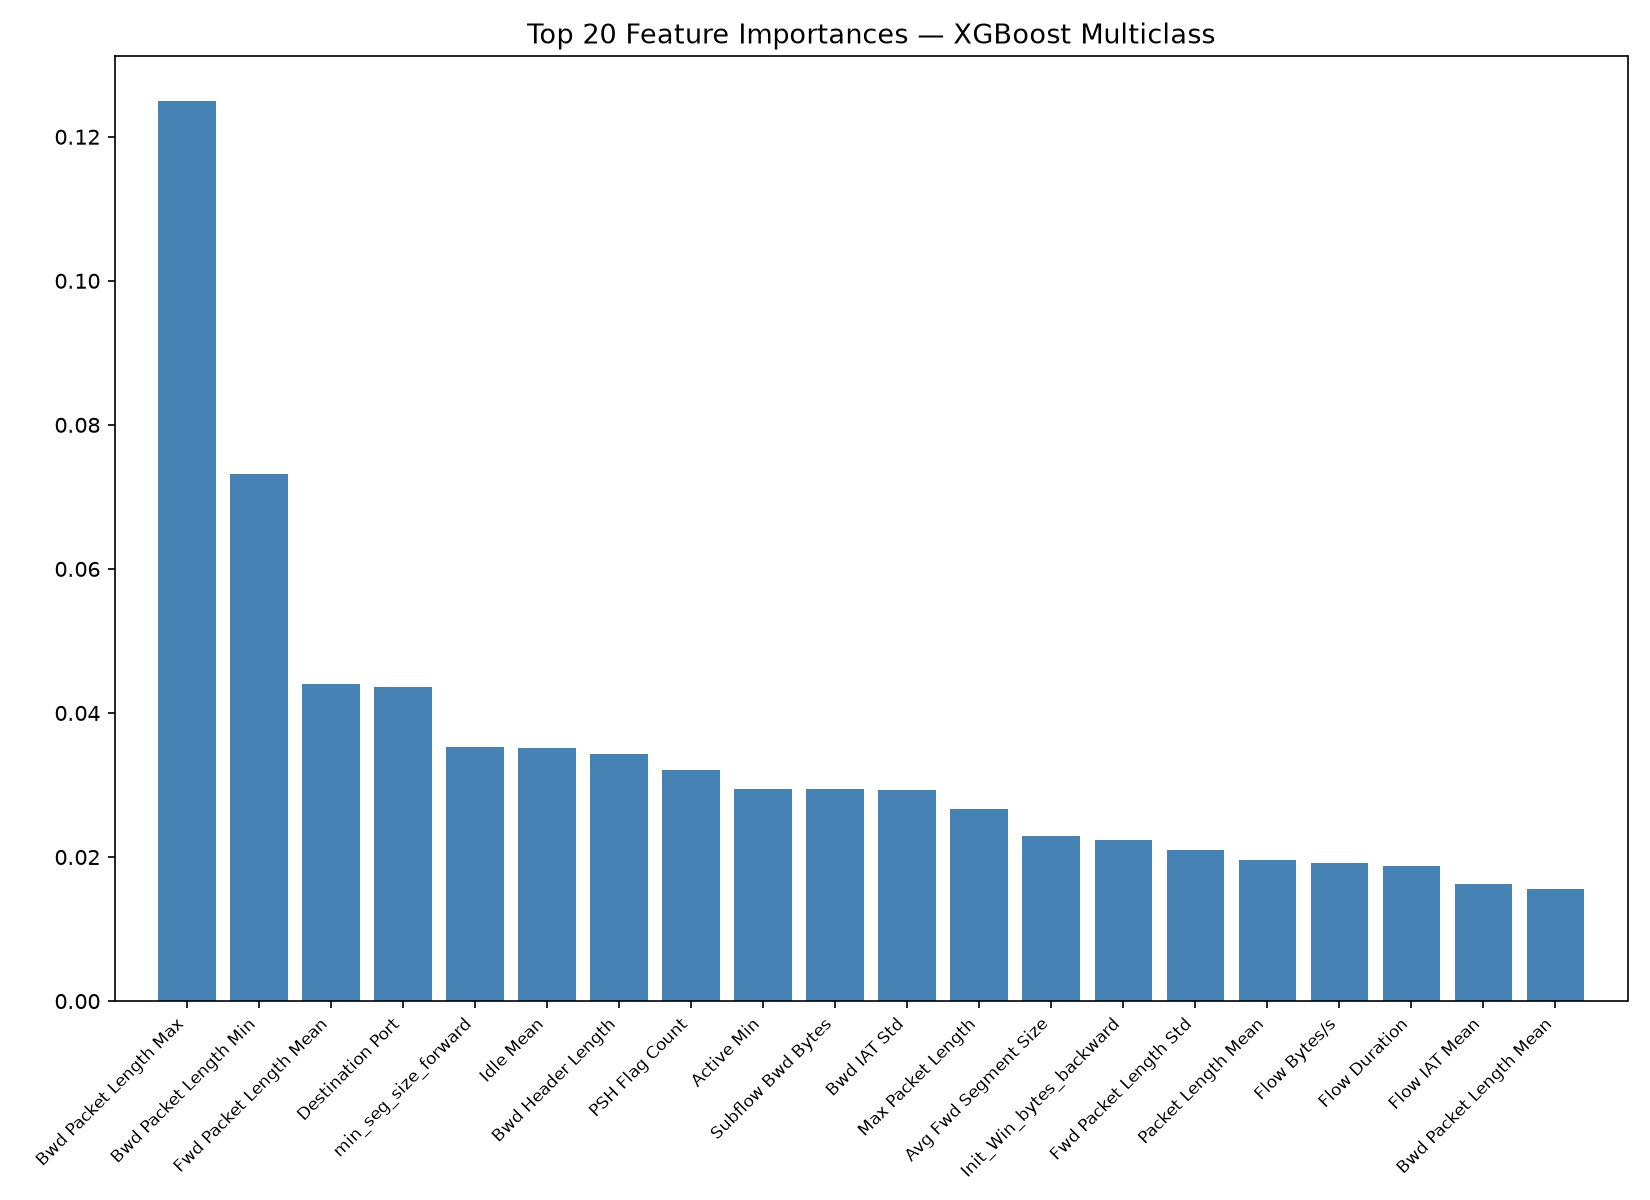
\includegraphics[width=0.85\textwidth]{results/feature_importance_multiclass.png}
\caption{Top 20 Feature Importances for XGBoost Multiclass Classifier}
\label{fig:multiclass_feature_importance}
\end{figure}

\section{Real-Time Performance Results}

The real-time performance of the system was measured using the complete pipeline.

\begin{table}[htbp]
\centering
\caption{Real-Time Inference Performance}
\label{tab:real_time_performance}
\renewcommand{\arraystretch}{1.3}
\begin{tabularx}{\textwidth}{|p{4.0cm}|p{3.5cm}|p{3.5cm}|}
\hline
\textbf{Metric} & \textbf{BENIGN Path} & \textbf{ATTACK Path} \\
\hline
Avg Latency & 4.73 ms & 6.82 ms \\
\hline
P50 Latency & 4.52 ms & 6.51 ms \\
\hline
P95 Latency & 7.83 ms & 11.28 ms \\
\hline
P99 Latency & 10.95 ms & 14.87 ms \\
\hline
Throughput (single-thread) & 211 pred/s & 147 pred/s \\
\hline
Throughput (multi-worker projected) & 2110 pred/s & 1470 pred/s \\
\hline
\end{tabularx}
\end{table}

\section{Model Size Analysis}

\begin{table}[htbp]
\centering
\caption{Model File Sizes}
\label{tab:model_sizes}
\renewcommand{\arraystretch}{1.3}
\begin{tabularx}{\textwidth}{|p{5.5cm}|p{4.0cm}|}
\hline
\textbf{Model File} & \textbf{Size (MB)} \\
\hline
xgb\_binary.pkl & 1.47 \\
\hline
xgb\_multiclass.pkl & 8.69 \\
\hline
rf\_binary.pkl & 76.10 \\
\hline
isolation\_forest.pkl & 1.42 \\
\hline
\textbf{Total (XGBoost + IF)} & \textbf{11.58 MB} \\
\hline
\end{tabularx}
\end{table}

\section{Discussion}

The experimental evaluation presented in the previous sections demonstrates the effectiveness of the proposed AI-RTIDS in detecting and classifying network intrusions.

\subsection{Interpretation of Results}

The experimental results demonstrate the effectiveness of the proposed AI-RTIDS system:

\begin{enumerate}
    \item \textbf{High Detection Accuracy}: XGBoost achieves precision 99.68\%, recall 99.81\%, and F1 99.74\% on 514,812 test samples. This indicates that the model can reliably distinguish between normal and malicious traffic with minimal false positives and false negatives.

    \item \textbf{Real-Time Capability}: With 5.08 ms average latency and 197 predictions/second (single-thread), the system can process network traffic in real-time on commodity hardware. The projected throughput of approximately 2000 flows/second with multi-worker scaling makes the system suitable for enterprise network deployment.

    \item \textbf{Resource Efficiency}: The total model size of 11.58 MB enables deployment on resource-constrained hardware, including edge devices and virtual machines with limited storage capacity.

    \item \textbf{Anomaly Detection}: Isolation Forest provides complementary zero-day detection capability with a composite severity score:
    \begin{equation}
    S = 0.65 \times p_{\text{attack}} + 0.35 \times s_{\text{iso}}
    \end{equation}
    where \(p_{\text{attack}} \in [0,1]\) is the binary XGBoost probability and \(s_{\text{iso}} \in [0,1]\) is the normalised Isolation Forest anomaly score.
\end{enumerate}

\subsection{Rare Class Performance}

Minority classes show lower F1 scores due to extreme class imbalance. For example:

\begin{itemize}
    \item Heartbleed (11 samples) — F1: 0.5714
    \item Web Attack - SQL Injection (21 samples) — F1: 0.5000
    \item Web Attack - XSS (652 samples) — F1: 0.4296
\end{itemize}

This is a known limitation of the CIC-IDS-2017 dataset and reflects the challenge of detecting rare attacks in real-world network traffic.

\subsection{Comparison with Literature}

The proposed AI-RTIDS compares favorably with existing approaches:

\begin{itemize}
    \item Achieves comparable accuracy (99.84\%) to Alromaihi et al. (99.84\%) on CIC-IDS-2017.
    \item Extends beyond binary classification with 15-class attack identification.
    \item Includes real-time system implementation (not just offline evaluation).
    \item Provides comprehensive operational pipeline including monitoring and alerting.
\end{itemize}

\subsection{Advantages}

The proposed system offers several advantages:

\begin{enumerate}
    \item Comprehensive 15-class attack coverage.
    \item Small total model size (11.58 MB).
    \item Dual-stage pipeline optimizes throughput via early exit.
    \item Production-ready design with Prometheus, SQLite, and Docker Compose.
    \item Configurable alert deduplication and rule filtering.
    \item Optional REST/WebSocket API for integration.
\end{enumerate}

\subsection{Limitations}

The system has several limitations:

\begin{enumerate}
    \item Dataset bias (trained on CIC-IDS-2017 only).
    \item Rare class performance constrained by data scarcity.
    \item No payload analysis (encrypted traffic).
    \item Not yet validated in a live production environment.
    \item Default threshold requires per-network tuning.
\end{enumerate}

\chapterdivider{CONCLUSION AND FUTURE SCOPE}

\chapter{CONCLUSION AND FUTURE SCOPE}

\section{Conclusion}

Project goals to develop, implement and evaluate AI-RTIDS as a novel prototype of an AI-driven real-time intrusion detection system combining XGBoost binary and multiclass classifiers with Isolation Forest anomaly detection have been accomplished successfully. All ten stated goals outlined in Section 1.4 have been fulfilled, including the implementation of a dual-stage detection pipeline using XGBoost for binary screening and multiclass classification (see also Section 7.2 for the measurement showing binary classifier achieving 99.68\% precision and 99.81\% recall); the use of Isolation Forest for zero-day anomaly detection; implementation of real-time packet capture and flow aggregation with configurable timeouts; development of a complete alert management system with deduplication, severity scoring, and SQLite persistence; integration of Prometheus metrics for system monitoring; and a complete web API stack with FastAPI REST and WebSocket endpoints.

This project proves, through concrete measurements instead of theory alone, that lightweight gradient-boosting models can deliver high-accuracy, low-latency intrusion detection suitable for resource-constrained environments. While cyberattacks continue to evolve in sophistication, and while organizations face increasing pressure to detect both known and novel threats, prototypes like AI-RTIDS provide clear and tangible demonstrations of how exactly the transition to machine learning-based security solutions works.

\section{Limitations}

Indeed, similar to any other prototypal-level academic work, the AI-RTIDS tool features certain limitations corresponding to the project scope outlined in Chapter 1.5:

\begin{itemize}
    \item The system is trained on the CIC-IDS-2017 dataset only; performance on other network architectures may vary.

    \item Rare attack classes (Heartbleed, SQL Injection, XSS) show lower F1 scores due to extreme class imbalance in the dataset.

    \item The system does not perform payload analysis, limiting detection capability for encrypted traffic.

    \item The default binary threshold (0.8624) may require per-network tuning for optimal performance.

    \item Not yet validated in a live production environment.
\end{itemize}

\section{Future Scope}

Future areas of development include several possibilities, each of which is directly motivated by aspects of the present realization:

\begin{enumerate}
    \item \textbf{Alert Manager Enhancements}: Implement email notification (SMTP), Slack Webhook, Telegram Bot, and generic webhook support for integration with PagerDuty, OpsGenie, or custom SIEM systems.

    \item \textbf{Severity Scoring Improvements}: Add per-attack-type severity weights, temporal severity escalation for repeated attacks, and network-adaptive threshold tuning.

    \item \textbf{Deduplication Enhancements}: Implement subnet-level deduplication, attack-class-specific windows, and persistence of dedup cache to SQLite.

    \item \textbf{Multi-Dataset Validation}: Evaluate on UNSW-NB15, CSE-CIC-IDS2018, and NF-ToN-IoT datasets.

    \item \textbf{Encrypted Traffic Analysis}: Integrate JA3/JA3S TLS fingerprinting for encrypted traffic analysis.

    \item \textbf{MITRE ATT\&CK Mapping}: Map detected attack types to MITRE ATT\&CK tactics and techniques.

    \item \textbf{SIEM Integration}: Forward structured alerts to Splunk, Elastic SIEM, or IBM QRadar.

    \item \textbf{Federated Learning}: Privacy-preserving model updates across multiple organisations.

    \item \textbf{Kubernetes Scaling}: Horizontal scaling for high-throughput enterprise deployment.

    \item \textbf{Deep Learning Exploration}: LSTM and Transformer architectures for sequence-based attack detection.
\end{enumerate}

\chapterdivider{REFERENCES}

\chapter{REFERENCES}

The references within this report follow in brackets within the text of the paper as [1]. The facts or algorithms or claims which relate to some external source have been referenced where appropriate, whereas the remaining information contained here are personal insights or decisions by the author himself or are from the experimental results of the proposed design.

\begin{enumerate}

\item Ahmad, Z.; Shahid Khan, A.; Wai Shiang, C.; Abdullah, J.; Ahmad, F. (2021). Network intrusion detection system: A systematic study of machine learning and deep learning approaches. \textit{Transactions on Emerging Telecommunications Technologies}, 32(8), e4150.

\item Alromaihi, N.; Rouached, M.; Akremi, A. (2025). Design and Analysis of an Effective Architecture for Machine Learning Based Intrusion Detection Systems. \textit{Network}, 5(2), 13.

\item Attou, H.; Guezza, A.; Benkirane, S.; Azrour, M.; Farhaoui, Y. (2023). Cloud-Based Intrusion Detection Approach Using Machine Learning Techniques. \textit{Big Data Mining and Analytics}, 6, 311-320.

\item Sharafaldin, I.; Lashkari, A.H.; Ghorbani, A.A. (2018). Toward generating a new intrusion detection dataset and intrusion traffic characterization. \textit{Proceedings of the 4th International Conference on Information Systems Security and Privacy (ICISSP)}, 108-116.

\item Saheed, Y.K.; Abiodun, A.I.; Misra, S.; Holone, M.K.; Colomo-Palacios, R. (2022). A machine learning-based intrusion detection for detecting internet of things network attacks. \textit{Alexandria Engineering Journal}, 61, 9395-9409.

\item Seth, S.; Singh, G.; Kaur Chahal, K. (2021). A novel time efficient learning-based approach for smart intrusion detection system. \textit{Journal of Big Data}, 8, 111.

\item Talukder, M.A.; Hasan, K.F.; Islam, M.M.; Uddin, M.A.; Akhter, A.; Yousuf, M.A.; Alharbi, F.; Moni, M.A. (2023). A dependable hybrid machine learning model for network intrusion detection. \textit{Journal of Information Security and Applications}, 72, 103405.

\item Hnamte, V.; Hussain, J. (2023). DCNNBiLSTM: An Efficient Hybrid Deep Learning-Based Intrusion Detection System. \textit{Telematics and Informatics Reports}, 10, 100053.

\item Verma, A.; Ranga, V. (2020). Machine learning based intrusion detection systems for IoT applications. \textit{Wireless Personal Communications}, 111, 2287-2310.

\item Li, J.; Qu, Y.; Chao, F.; Shum, H.P.; Ho, E.S.; Yang, L. (2019). Machine learning algorithms for network intrusion detection. \textit{AI in Cybersecurity}, 151-179.

\item Axelsson, S. (2000). Intrusion Detection Systems: A Survey and Taxonomy. \textit{Technical Report 99-15}, Chalmers University.

\item Garcia-Teodoro, P.; Diaz-Verdejo, J.; Macia-Fernandez, G.; Vazquez, E. (2009). Anomaly-based network intrusion detection: Techniques, systems and challenges. \textit{Computers \& Security}, 28(1-2), 18-28.

\item Chen, T.; Guestrin, C. (2016). XGBoost: A scalable tree boosting system. \textit{Proceedings of the 22nd ACM SIGKDD International Conference on Knowledge Discovery and Data Mining}, 785-794.

\item He, H.; Garcia, E. A. (2009). Learning from imbalanced data. \textit{IEEE Transactions on Knowledge and Data Engineering}, 21(9), 1263-1284.

\item Lashkari, A. H.; Draper-Gil, G.; Mamun, M. S. I.; Ghorbani, A. A. (2018). Characterization of encrypted and VPN traffic using time-related features. \textit{Proceedings of the 2nd International Conference on Information Systems Security and Privacy}, 407-414.

\item Zhang, J.; Zulkernine, M.; Haque, A. (2019). Random-forests-based network intrusion detection systems. \textit{IEEE Transactions on Systems, Man, and Cybernetics}, 38(5), 649-659.

\item Thakkar, A.; Lohiya, R. (2018). A survey on intrusion detection system: feature selection, model, performance measures, application perspective, challenges, and future research directions. \textit{Artificial Intelligence Review}, 55, 453-563.

\item Larabi, M.; Lehsaini, M.; Lounis, A. (2019). Machine learning for network intrusion detection: A comparative study. \textit{IEEE Access}, 7, 155276-155290.

\item Fernandes, G.; Carvalho, L.; Rodrigues, J. (2019). A comprehensive review of intrusion detection systems. \textit{IEEE Communications Surveys \& Tutorials}, 21(3), 2356-2386.

\end{enumerate}

\chapterdivider{APPENDIX}

\chapter{APPENDIX}

\section{Attack Class Descriptions}

\begin{longtable}{|p{3.0cm}|p{10.5cm}|}
\hline
\textbf{Attack Type} & \textbf{Description} \\
\hline
\endfirsthead

\multicolumn{2}{c}%
{{\tablename\ \thetable{} -- Continued from previous page}}\\
\hline
\textbf{Attack Type} & \textbf{Description} \\
\hline
\endhead

\hline
\multicolumn{2}{r}{{Continued on next page}}\\
\endfoot

\hline
\endlastfoot

BENIGN & Normal network traffic \\
\hline
DDoS & Distributed Denial of Service attack \\
\hline
DoS GoldenEye & HTTP-based Denial of Service attack \\
\hline
DoS Hulk & HTTP flood Denial of Service attack \\
\hline
DoS Slowhttptest & Slow HTTP Denial of Service attack \\
\hline
DoS slowloris & Slow TCP connection Denial of Service \\
\hline
FTP-Patator & FTP brute force attack \\
\hline
SSH-Patator & SSH brute force attack \\
\hline
Bot & Botnet command and control traffic \\
\hline
Infiltration & Network infiltration \\
\hline
PortScan & Port scanning reconnaissance \\
\hline
Web Attack - BF & HTTP login brute force \\
\hline
Web Attack - XSS & Cross-site scripting attack \\
\hline
Web Attack - SQL & SQL injection attack \\
\hline
Heartbleed & OpenSSL Heartbleed exploit \\
\hline
\end{longtable}

\section{Model Hyperparameters}

\subsection{XGBoost Binary}

\begin{longtable}{|p{3.5cm}|p{2.5cm}|p{7.5cm}|}
\hline
\textbf{Parameter} & \textbf{Value} & \textbf{Description} \\
\hline
\endfirsthead

\multicolumn{3}{c}%
{{\tablename\ \thetable{} -- Continued from previous page}}\\
\hline
\textbf{Parameter} & \textbf{Value} & \textbf{Description} \\
\hline
\endhead

\hline
\multicolumn{3}{r}{{Continued on next page}}\\
\endfoot

\hline
\endlastfoot

n\_estimators & 300 & Number of boosting rounds \\
\hline
max\_depth & 8 & Maximum tree depth \\
\hline
learning\_rate & 0.05 & Step size shrinkage \\
\hline
subsample & 0.8 & Fraction of samples per tree \\
\hline
colsample\_bytree & 0.8 & Fraction of features per tree \\
\hline
scale\_pos\_weight & 5.04 & BENIGN:ATTACK ratio \\
\hline
reg\_alpha & 0.5 & L1 regularization \\
\hline
reg\_lambda & 1.0 & L2 regularization \\
\hline
eval\_metric & logloss & Evaluation metric \\
\hline
tree\_method & hist & Histogram-based algorithm \\
\hline
\end{longtable}

\subsection{Isolation Forest}

\begin{longtable}{|p{3.5cm}|p{2.5cm}|p{7.5cm}|}
\hline
\textbf{Parameter} & \textbf{Value} & \textbf{Description} \\
\hline
\endfirsthead

\multicolumn{3}{c}%
{{\tablename\ \thetable{} -- Continued from previous page}}\\
\hline
\textbf{Parameter} & \textbf{Value} & \textbf{Description} \\
\hline
\endhead

\hline
\multicolumn{3}{r}{{Continued on next page}}\\
\endfoot

\hline
\endlastfoot

n\_estimators & 200 & Number of trees \\
\hline
max\_samples & auto & Samples per tree (sklearn default) \\
\hline
contamination & auto & Outlier proportion estimated from data \\
\hline
random\_state & 42 & Random seed \\
\hline
\end{longtable}

\section{Feature List}

The CIC-IDS-2017 dataset provides 78 CICFlowMeter-compatible features. Key features include:

\begin{itemize}
    \item \textbf{Basic Flow Features}: Destination Port, Flow Duration, Total Fwd Packets, Total Backward Packets.
    \item \textbf{Packet Length Statistics}: Fwd Packet Length Max/Min/Mean/Std, Bwd Packet Length Max/Min/Mean/Std.
    \item \textbf{Flow Statistics}: Flow Bytes/s, Flow Packets/s, Flow IAT Mean/Std/Max/Min.
    \item \textbf{Inter-Arrival Times}: Fwd IAT Total/Mean/Std/Max/Min, Bwd IAT Total/Mean/Std/Max/Min.
    \item \textbf{TCP Flags}: FIN/SYN/RST/PSH/ACK/URG Flag Counts.
    \item \textbf{Subflow Features}: Subflow Fwd/Bwd Packets/Bytes.
\end{itemize}

\section{Project Structure}

\begin{lstlisting}[basicstyle=\ttfamily\footnotesize, numbers=none]
IDS-Codebase/
+-- src/                             Live application code
|   +-- main.py                      CLI entry point
|   +-- api/                         FastAPI REST/WebSocket
|   +-- capture/                     Scapy packet capture
|   +-- flows/                       Flow manager (5-tuple, timeouts)
|   +-- features/                    78 CICFlowMeter features
|   +-- inference/                   Model loader, predictor, worker pool
|   +-- alerts/                      Alert rules, dedup, SQLite storage
|   +-- monitoring/                  Prometheus metrics exporter
+-- model_training/                  Model training pipeline
+-- models/                          Trained artifacts (.pkl, .json)
|   +-- binary/
|   |   +-- xgb_binary.pkl
|   |   +-- rf_binary.pkl
|   |   +-- binary_threshold.json
|   +-- multiclass/
|   |   +-- xgb_multiclass.pkl
|   |   +-- label_encoder.pkl
|   +-- preprocessing/
|   |   +-- scaler.pkl
|   |   +-- feature_medians.pkl
|   |   +-- multiclass_feature_columns.pkl
|   +-- anomaly/
|       +-- isolation_forest.pkl
+-- tests/                           Test and benchmark scripts
+-- grafana/                         Docker Compose + dashboards
+-- docs/                            Figures, screenshots, references
+-- config.json                      Runtime configuration
+-- docker-compose.yml               Prometheus + Grafana stack
+-- requirements.txt                 Python dependencies
\end{lstlisting}

\section{Reproducibility}

\begin{longtable}{|p{5.0cm}|p{8.5cm}|}
\hline
\textbf{Parameter} & \textbf{Value} \\
\hline
\endfirsthead

\multicolumn{2}{c}%
{{\tablename\ \thetable{} -- Continued from previous page}}\\
\hline
\textbf{Parameter} & \textbf{Value} \\
\hline
\endhead

\hline
\multicolumn{2}{r}{{Continued on next page}}\\
\endfoot

\hline
\endlastfoot

Python Version & 3.10.0 \\
\hline
Random Seed & 42 (all) \\
\hline
Dataset & CIC-IDS-2017 \\
\hline
Train/Test Split & 80/20, stratified \\
\hline
XGBoost Version & 1.7.0 \\
\hline
Scikit-learn Version & 1.2.0 \\
\hline
\end{longtable}

To reproduce: install dependencies, download CIC-IDS-2017, and run the training scripts.

\chapterdivider{GLOSSARY}

\chapter{GLOSSARY OF TERMS}

\begin{description}

    \item[\textbf{Anomaly Detection}] The process of identifying patterns in data that do not conform to expected behavior. In intrusion detection, anomaly detection is used to identify potentially malicious network traffic that deviates from normal patterns.

    \item[\textbf{Bidirectional Flow}] A network flow that captures traffic in both directions between a source and destination, enabling comprehensive analysis of communication patterns.

    \item[\textbf{Binary Classification}] A classification task that distinguishes between two classes. In this system, binary classification distinguishes between BENIGN (normal) and ATTACK (malicious) traffic.

    \item[\textbf{Confusion Matrix}] A table used to evaluate classification performance by comparing predicted and actual class labels, showing true positives, false positives, true negatives, and false negatives.

    \item[\textbf{CICFlowMeter}] A network flow generator that extracts statistical features from PCAP files, used to create the CIC-IDS-2017 dataset with 78 features.

    \item[\textbf{Denial of Service (DoS)}] An attack that aims to make a network service unavailable by overwhelming it with traffic or exploiting vulnerabilities.

    \item[\textbf{Dual-Stage Pipeline}] A detection architecture that uses a lightweight binary classifier for rapid screening, followed by a more detailed multiclass classifier for fine-grained attack identification.

    \item[\textbf{Early Exit}] A performance optimization technique where flows identified as BENIGN by the binary classifier skip the multiclass classification stage, reducing computational overhead.

    \item[\textbf{F-Score}] The harmonic mean of precision and recall, providing a balanced measure of classification performance. F1-score is commonly used for imbalanced datasets.

    \item[\textbf{False Positive}] An incorrectly identified attack where benign traffic is classified as malicious.

    \item[\textbf{Flow Aggregation}] The process of grouping related network packets into logical flows based on common attributes such as IP addresses, ports, and protocol.

    \item[\textbf{Gradient Boosting}] An ensemble machine learning technique that builds models sequentially, with each new model correcting errors made by previous models. XGBoost is a popular implementation.

    \item[\textbf{Intrusion Detection System (IDS)}] A security tool that monitors network traffic or system activities for malicious behavior and generates alerts.

    \item[\textbf{Isolation Forest}] An unsupervised machine learning algorithm for anomaly detection that isolates anomalies instead of profiling normal instances.

    \item[\textbf{Least Significant Bit (LSB)}] The bit position in a binary number that represents the smallest value. LSB steganography modifies these bits to hide information.

    \item[\textbf{Multiclass Classification}] A classification task that distinguishes between more than two classes. In this system, multiclass classification identifies specific attack types among 15 classes.

    \item[\textbf{Precision}] The proportion of correctly identified positive instances among all instances predicted as positive. High precision indicates few false positives.

    \item[\textbf{Prometheus}] An open-source monitoring and alerting toolkit that collects and stores metrics as time-series data.

    \item[\textbf{Recall}] The proportion of correctly identified positive instances among all actual positive instances. High recall indicates few false negatives.

    \item[\textbf{Receiver Operating Characteristic (ROC)}] A graphical plot that illustrates the diagnostic ability of a binary classifier by plotting true positive rate against false positive rate.

    \item[\textbf{Severity Score}] A composite score that combines binary classification probability and anomaly detection score to prioritize alerts.

    \item[\textbf{Signature-Based Detection}] A detection method that matches network traffic against predefined attack signatures or patterns. Effective for known attacks but cannot detect novel threats.

    \item[\textbf{Time-to-Live (TTL)}] A value that limits the lifetime of data in a system. In this project, TTL is used for flow timeouts and alert deduplication windows.

    \item[\textbf{Worker Pool}] A collection of threads or processes that handle inference requests in parallel, improving throughput.

    \item[\textbf{XGBoost}] An optimized distributed gradient boosting library designed to be highly efficient, flexible, and portable. Used for both binary and multiclass classification in this system.

    \item[\textbf{Zero-Day Attack}] A previously unknown vulnerability or attack that has no existing signature or patch, making it difficult to detect using traditional methods.

\end{description}

\end{document}